\documentclass[floatsintext, man]{apa6}
%\bibliography{references}
\usepackage{apacite}
\usepackage{subcaption}
\usepackage{booktabs}
\usepackage{xspace}
\usepackage[utf8]{inputenc}
\usepackage{amsmath}
\usepackage{amssymb}
\usepackage{tikz}
%\usepackage[sc,osf]{mathpazo}
%\linespread{1.12}
\usepackage{booktabs}
\usepackage{centernot}
\usepackage{tabularx}
\usepackage{tikz}
% \usepackage{subfigure}
\usetikzlibrary{bayesnet}


  \def\firstcircle{(90:1cm) circle (1.5cm)}
  \def\secondcircle{(210:1cm) circle (1.5cm)}
  \def\thirdcircle{(330:1cm) circle (1.5cm)}
  
  
  %\draw (0,0) circle (1) (-0.5,0.25)  node [text=black,above] {$A$}
%      (1,0) circle (1) (1.5, 0.25)  node [text=black,above] {$B$}
%      (0.5,-1) circle (1) (0.5,-1.25)  node [text=black,below] {$C$}
%      (-1.5,-2.25) rectangle (2.5,1.25) node [text=black,above] {};

% these packages are needed to insert results 
% obtained from R into the LaTeX document
\usepackage{pgfplotstable}
\usepackage{csvsimple}
\usepackage{siunitx}

% set the name of the folder in which the CSV files with 
% information from R is stored
\newcommand{\datafoldername}{csv_to_tex}


%\makeatletter
%    \let\@internalcite\cite
%    \def\cite{\def\citeauthoryear##1##2{##1, ##2}\@internalcite}
%    \def\shortcite{\def\citeauthoryear##1{##2}\@internalcite}
%    \def\@biblabel#1{\def\citeauthoryear##1##2{##1, ##2}[#1]\hfill}
%\makeatother


% the following code defines the convenience functions
% as described in the main text below

% rlgetvalue returns whatever is the in cell of the CSV file
% be it string or number; it does not format anything
\newcommand{\rlgetvalue}[4]{\csvreader[filter strcmp={\mykey}{#3},
             late after line = {{,}\ }, late after last line = {{}}]
            {\datafoldername/#1}{#2=\mykey,#4=\myvalue}{\myvalue}}

% rlgetvariable is a shortcut for a specific CSV file (myvars.csv) in which
% individual variables that do not belong to a larger chunk can be stored
\newcommand{\rlgetvariable}[1]{\csvreader[]{\datafoldername/myvars.csv}{#1=\myvar}{\myvar}\xspace}

% rlnum format a decimal number
\newcommand{\rlnum}[2]{\num[output-decimal-marker={.},
                             exponent-product = \cdot,
                             round-mode=places,
                             round-precision=#2,
                             group-digits=false]{#1}}

\newcommand{\rlnumsci}[2]{\num[output-decimal-marker={.},
                          scientific-notation = true,
                             exponent-product = \cdot,
                             round-mode=places,
                             round-precision=#2,
                             group-digits=false]{#1}}

\newcommand{\rlgetnum}[5]{\csvreader[filter strcmp={\mykey}{#3},
             late after line = {{,}\ }, late after last line = {{}}]
            {\datafoldername/#1}{#2=\mykey,#4=\myvalue}{\rlnum{\myvalue}{#5}}}

\newcommand{\rlgetnumsci}[5]{\csvreader[filter strcmp={\mykey}{#3},
             late after line = {{,}\ }, late after last line = {{}}]
            {\datafoldername/#1}{#2=\mykey,#4=\myvalue}{\rlnumsci{\myvalue}{#5}}}



\makeatletter
\patchcmd{\epigraph}{\@epitext{#1}}{\itshape\@epitext{#1}}{}{}
\makeatother \def\signed
#1{{\leavevmode\unskip\nobreak\hfil\penalty50\hskip2em
\hbox{}\nobreak\hfil#1% \parfillskip=0pt \finalhyphendemerits=0
\endgraf}} \newsavebox\mybox 

\newenvironment{aquote}[1]
{\savebox\mybox{#1}\begin{quote}} {\signed{\usebox\mybox}\end{quote}}

%\newcommand{\HRule}{\rule{\linewidth}{0.2mm}}



\title{Logic, probability, and pragmatics in syllogistic reasoning}
\shorttitle{Pragmatics in Syllogistic Reasoning}

\author{Michael Henry Tessler\textsuperscript{1}\textsuperscript{,2}, Joshua B. Tenenbaum\textsuperscript{1},~and \\Noah D. Goodman\textsuperscript{2}}
\date{}
  
\affiliation{
\vspace{0.5cm}
\textsuperscript{1} Department of Brain and Cognitive Sciences, Massachusetts Institute of Technology \\
\textsuperscript{2} Department of Psychology, Stanford University
}
%\authorsnames[{1,2},1,2]{Michael Henry Tessler, Joshua B. Tenenbaum, Noah D. Goodman}
%\authorsaffiliations{{Department of Brain and Cognitive Sciences, MIT}, {Department of Psychology, Stanford University}}

\date{}

\usepackage{xcolor}
\usepackage{bbm}

\newcommand{\denote}[1]{\mbox{ $[\![ #1 ]\!]$}}
\newcommand*\diff{\mathop{}\!\mathrm{d}}
\definecolor{Red}{RGB}{255,0,0}
\definecolor{Green}{RGB}{10,200,100}
\definecolor{Blue}{RGB}{10,100,200}

\newcommand{\mht}[1]{{\textcolor{Blue}{[mht: #1]}}}
\newcommand{\ndg}[1]{{\textcolor{Green}{[ndg: #1]}}}
\newcommand{\red}[1]{{\textcolor{Red}{#1}}}

\authornote{Corresponding author: Michael Henry Tessler,  Department of Brain and Cognitive Sciences, Building 46, Room 3027,	Massachusetts Institute of Technology, 77 Massachusetts Avenue, Cambridge, MA 02139-4307, USA; tessler@mit.edu}

\keywords{syllogisms; reasoning; pragmatics; semantics; Rational Speech Act \newline\indent Word count: 6639}

\abstract{
Syllogistic reasoning lies at the intriguing intersection of natural and formal reasoning, of language and logic. 
Syllogisms comprise a formal system of reasoning yet make use of natural language quantifiers (e.g., \emph{all}, \emph{some}), and invite natural language conclusions. 
The conclusions people tend to draw from syllogisms deviate substantially from a purely logical perspective. 
Are principles of natural language understanding to blame?
We develop probabilistic pragmatics models of syllogistic reasoning, couched within the Rational Speech Act framework, and explore the pressures that pragmatic reasoning place on the production of conclusions.
We test our models on a recent, large data set of syllogistic reasoning and find that reasoners select conclusions in a pragmatic manner with the goal of aligning the beliefs of a naive listener to those of their own. 
We compare our model to previously published models that implement two alternative theories -- Mental Models and Probability Heuristics -- finding that our model accounts for the full distributions of responses in a manner slightly better than previous accounts but with an order-of-magnitude fewer parameters. 
Our approach represents a view of human syllogistic reasoning as natural communication.}
% 6639

\begin{document}
\maketitle


%\begin{aquote}{\textbf{Walter J. Ong}, \emph{Orality and Literacy} (1982)}The syllogism is like a text: fixed, boxed-off, isolated... The riddle [by contrast] belongs in the oral world. To solve a riddle, canniness is needed: one draws on knowledge, often deeply subconscious, beyond the words themselves in the riddle. \end{aquote}

%\HRule

\newpage

\section{Introduction}

Imagine discussing a recent tax proposal TR158 with a friend. Your friend remarks that in TR158:

\begin{quote}
Some of the taxes on the wealthy will be modified. \\
All of the tax modifications in the bill will expire in 10 years.
\end{quote}

From these remarks, it follows -- logically, necessarily -- that \emph{Some of the tax modifications on the wealthy will expire in 10 years}.
That is, in all situations in which the premises are true, the conclusion is also true. 
The argument is logically valid.
Now consider a superficially similar set of remarks: In TR158,

\begin{quote}
All of the taxes on the wealthy will be modified. \\
Some of the tax modifications in the bill will expire in 10 years.
\end{quote}

You may be tempted to draw a similar conclusion:  \emph{Some of the tax modifications on the wealthy will expire in 10 years}.
The argument seems reasonable, and yet the conclusion is not true in all situations in which the premises are true.
The argument is logically invalid.
Consider, for instance, that there could be tax modifications applied to the non-wealthy, and that those modifications are the ones that will expire in 10 years.


Human intuitions about what conclusions reasonably follow from a set of premises are seemingly supported by something other than pure logical necessity. %, then what is that?
Aristotle's invention of syllogisms -- the kinds of two premise arguments shown above --  can be interpreted, in fact, as an attempt to tame the irrationality of the human mind.
% Syllogisms are the foundation of modern logic.
In recent centuries, cognitive psychologists have turned the syllogism back on the human mind, as a rational basis from which to evaluate human reasoning \cite{Storring1908}.
Perhaps unsurprisingly, how everyday human beings reason with syllogisms differs from what classical rules of logic would dictate \cite<for a meta-analysis, see:>{Khemlani2012}.



%For as long as humans having been thinking about thinking (at least in the Western tradition), they have been thinking about logical arguments like the one above, known as syllogisms.
% Aristotle developed syllogisms to articulate the conclusions which rationally follow from a set of premises, which cognitive psychologists took up to serve 
% Syllogisms thus also became one of the first domains where cognitive psychology looked to evaluate human reasoning against a set of rational norms.


Our modeling approach is a Computational or Rational Level of analysis model \cite{marr1982vision, anderson1990adaptive} that seeks to describe the computations that underly human syllogistic reasoning without stipulating a precise implementation of such a reasoning process. 



%We have a similar goal to PHM (rational analysis). 
%MMT is trying to do something different. 
A syllogism is a formal logical argument that uses quantifiers (e.g. \emph{all}, \emph{some}) to relate two properties (e.g., \emph{taxes on the wealthy} and \emph{expiring in 10 years}) via a third (``middle'') property (e.g., \emph{being modified by the proposal}). 
Many theoretical frameworks have been brought to explain how humans reason with syllogisms.
Logic or syntactic-based approaches have attempted to articulate modified logical rules -- so-called ``natural logic'' -- that humans deploy when evaluating syllogistic arguments \cite{braine1983logical, rips1994, geurts2003reasoning}.
% Semantic approaches have theorized about the 
Process accounts have been developed to describe how we manipulate  model- or diagram-based mental representations to arrive at a conclusion, the most prominent example being the Mental Models theory \cite{johnson1975models}.
Still other approaches attempt to articulate the rational or functional basis of human logical reasoning, interrogating deductive reasoning as a special case of probabilistic inference \cite{oaksford2001probabilistic, oaksford2007bayesian, hahn2007rationality, tenenbaum2006theory},  formalized in the Probability Heuristics Model of syllogistic reasoning \cite{Chater1999}.



%: both mm and ph take on a fairly standard  competence theory (FO logic, probability) but then have to appeal to process idiosyncrasies or heuristics, both thought to arise from resource constraints in order to explain human judgements. 


Though the substantial prior work provides insight into how humans reason with syllogisms, a unified, explanatory theory of human syllogistic reasoning remains outstanding \cite{Khemlani2012}. 
The most prominent accounts of syllogistic reasoning -- Mental Models Theory \cite{johnson1975models, johnson2015logic} and the Probability Heuristics Model  \cite{Chater1999} -- assume a standard competence-level theory involving first-order logic and probabilities, but appeal to either process-level idiosyncrasies or heuristics presumed to arise from resource constraints in order to explain human judgments. 
Furthermore, the fact that syllogisms involve natural language demands a theory that can be integrated with principles of natural language -- semantics and pragmatics -- which are intuitively at play for human reasoning \cite{sperber1986relevance,mercier2017enigma}.
Natural language semantics plays a role in many theories of reasoning \cite{JL1978, Khemlani2012, geurts2003reasoning}, but how those semantics interface with pragmatic reasoning is either posited in an ad-hoc manner \cite{Chater1999} or has been limited to simple Gricean enrichment of the premises \cite{Roberts2001}.	


%in contrast, we also start from FO logic with probabilities, but construe syllogistic reasoning as part of communication thus adding pragmatic conclusion selection as part of the competence theory. while there are almost certainly important processing details driven by resource limitations, we don't need to appeal to them in order to explain many aspects of human judgements.

We take up the task of developing a competence-level theory that builds upon first-order logic and probabilities but construes syllogistic reasoning as part of communication. 
%in the style of \citeA{marr1982vision} and \citeA{anderson1990adaptive} that integrates three core ingredients widely believed to be at play in human syllogistic reasoning: logic, probability, and pragmatics. 
%$ logic, probability, and pragmatics in a rational model.
%\mht{should start with more about probabilistic models and logic}
In particular, we view syllogistic reasoning through the lens of the language understanding processes that guide everyday reasoning with language, a process which involves reasoning about how an interlocutor would interpret a speaker's statements \cite{Grice1975, Clark1996, Levinson2000}. 
% interpreting the meanings of the sentences heard and social reasoning about why a speaker would bother to say those sentences 
% Syllogistic reasoning is then part logical reasoning and part riddle solving (as suggested by the Ong, 1982 quotation above).
%Each of these component tasks could involve pragmatic reasoning beyond the words of the syllogism 
We formalize this hypothesis in a probabilistic model of pragmatic reasoning in the Rational Speech Act framework \cite{Frank2012a, goodman2016pragmatic}.
Our model is able to explain a number of qualitative phenomena in syllogistic reasoning, including articulating a rational mechanism by which a person could respond \emph{nothing follows}, an outstanding problem in theories of syllogistic reasoning \cite{riesterer2020modeling}.
We additionally show that pragmatics enters into the conclusion selection process by way of participants reflecting on how well their choice of conclusion would convey their own beliefs to a naive listener. 
While there are almost certainly important processing details driven by resource limitations, we do not need to appeal to them in order to explain many aspects of human judgements.
And though we do not explain all of the variance in the human data, the model provides a path forward for addressing several outstanding issues including including how pragmatics might enter into the interpretation of premises and  how the content of a syllogism can affect reasoning (known as \emph{belief bias}).
%We discuss the question of whether premise interpretation may also be pragmatic in some important way.
%As a Bayesian model, our approach also naturally extends to explain



% thwhat is still outstanding is a model that unifies and explains syllogistic reasoning in terms of a rational computation.\ndg{i don;t think we want to say that...}
%The most promising application of explaining syllogistic reasoning in terms of a rational computation, the Probability Heuristics Model, falls short at fully articulating a coherent probabilistic logic and instead resorts to positing ad-hoc heuristics thought to approximate that logic \cite{Chater1999}.
%The mental models approach provides a process-level account, which can be enhanced with probabilistic constructs and assumptions \cite{johnson2015logic}, but does not have the goal of providing a rational analysis. 
% is still outstanding. 
%In particular, a model that tries to explain how reasoning works and why it fails 
% why mental reasoning works, what the function is, how it achieves that function, and how errors might arise from gaps between the problem the mind is solving and what the context might require.
%PHM -- doesn't provide a 
%
%
%-- rational analysis of syllogistic reasoning
%- explains what its for and why it works
%- the problem people are solving is communicating beliefs rather than deducing what is true


%Contra more traditional approaches that  assume deductive reasoning is the ideal framework by which to evaluate human reasoning  and try to explain reasoning errors as arising from improper use of deductive rules \cite{rips1994, geurts2003reasoning} or biased construction of logical models \cite{JL1984, Newstead1992}, the probabilisitic lens assumes that human reasoners about logical reasoning tasks as they approach many other kinds of everyday reasoning, which often takes the form of probabilistic inference under uncertainty \cite{tenenbaum2006theory}. 





%More recently, theorists have looked to a probability-based logic to develop hypotheses about how people reason with logic arguments \cite{Oaksford1994, oaksford2007bayesian, hahn2007rationality}, the flagship application of which is the Probability Heuristics model \cite{Chater1999}.
%In the background of most of this theoretical work as well is a consensus that communicative factors <e.g., pragmatic reasoning; >{sperber1986relevance,mercier2017enigma} play some role in syllogistic reasoning \cite{Roberts2001}.
%Still, a unified model for human reasoning with syllogisms remains out of reach \cite{Khemlani2012}.
%Though attempts have been made to bring some of these factors together \cite{johnson2015logic}, integrating logic and probability into a rational model and formalizing how communicative factors could manifest in syllogistic reasoning has not yet been achieved. 



%The idealized logical and/or probabilistic framework in which thinking and reasoning unfolds is just part of process of syllogistic reasoning, however. 
%Syllogisms comprise a formal logical system, but they are expressed using the tools of natural language (e.g., natural language quantifiers).
%Reasoning through a syllogism, thus, involves interpreting and producing natural language sentences; understanding such a task requires a careful examination of the  that may be at play.

% Inspired by Luria's experiments, we explore the idea that understanding human syllogistic reasoning requires a careful look at participants' understanding of the task \cite{henle1962relation}. 


%\ndg{say "rational" a lot less i this section.}

% How are people understanding the logic and what other kinds of processes may be going on?

%In all these cases, however, 
%Others have looked to the rational probabilistic based ]
%If people are not performing logical reasoning, however, then what they are doing when reasoning with syllogisms is not clear.

% What people are doing, however, if they are not doing logical reasoning has been contentious. 
%Syntactics, semantics of mental models, natural logic
% [before OC]
%There is no question that when people reason about syllogisms 
%
%
%What is reasoning?
%Dating back to at least Aristotle, humans have developed many different (formal) systems of reasoning.
%Some systems rely on the application of logical rules and others on probabilistic computations.
%On the other hand, human beings reason about concrete events that happen in the world.
%How do the formal systems we have for understanding reasoning relate to the human capacity for reasoning?


%Rationality debates 
%One of the very first places where what was of interest where people depart from rational norms.
%No question that people have a sense that when they reason about these problems, what seems the right conclusions is different from logicians.
%What people have been doing when reasoning about syllogisms is contentious. 
%
%
%Then we had the probabilistic turn.
%Even when you think you're doing deduction, you're doing some kind of probabilistic reasoning. 
%OC presents the climatic chapter.
%But it is not really climatic. relies upon heuristics.
%
%What are people really doing here? What else might they be doing? Communicative reasoning (sperber).
%What's likely to be true as well as what's actually true.
%
%We haven't had any models that bring these things together.
%Unpacking what are the kinds of rationality in human syllogistic reasoning.
%
%We havent solved this problem
%
%underlying logical semantics, in a probabilistic inference framework embedded
%
%able to explain the data qualitivalety and quantitatively better than previous model.
%the nothing follows thing.
%show the importance of each of these factors.
%
%we think it's an important step forward because of how it elucidates the contributions of logical, probability and pragmatics in this classic domain of reasoning. 
%
%other factors might be explained by noisy channel (?) or just irrationality. 




%A fundamental question in the study of human cognition is how the formal systems that humans have developed 
%
%
%In a famous scientific expedition of the 1930s, Russian psychologist Alexander Luria set off into the remote areas of Uzbekistan and Kyrgyzstan in the former Soviet Union to understand the minds of the illiterate peoples of Russia. Among his experiments, Luria would give his participants verbal reasoning problems such as the following:
%
%\begin{quote}
%In the Far North, where there is snow, all bears are white. \\
%Novaya Zembla is in the Far North and there is always snow there. \\
%What color are the bears?
%\end{quote}

%The literacy of Luria's participant was a large factor in the response he received.
%While a literate person responded logically (```...they should all be white''), a typical response from an illiterate participant would be: ``I don't know. I've seen a black bear. I've never seen any others. Each locality has its own animals'' \cite{luria1976cognitive}. 
%%Reasoning by appealing to experience or common knowledge, 
%Obviously, this is not the answer that Luria had in mind, but what would lead a person to respond in the way that this person did?

%The kind of response Luria received to such a question depended in part on the literacy of his participant. 
%A person who knew how to read and write would respond: ``To go by your words, they should all be white.''
%An illiterate person, on the other hand, would say: 

%Similar flavors of responses -- appealing to experience or background knowledge -- were found in classic anthropological studies with the Kpelle of Liberia \cite{cole1971cultural, scribner1975recall}.
% A study of American graduate students of the 1960s also uncovered erroneous judgments, and through an analysis of the written protocols of the participants, it was suggested that ``where error occurs, it need not involve faulty reasoning but may be a function of the individual's understanding of the task or materials presented to him'' \cite{henle1962relation}. 

%The problem Luria gave his participants resembles a syllogism: a two-sentence argument used to relate two properties (or terms: A, C) via a middle term (B). 
%
%\begin{figure}
%\begin{tabularx}{.8\textwidth}{XXXX}
%%\begin{quotation} 
%
%& & & \\
%\bf A \--- B & \bf B \--- A  & \bf A \--- B & \bf B \--- A \\
%\bf B \--- C & \bf C \--- B  & \bf C \--- B & \bf B \--- C \\
%\bf \textemdash & \textemdash & \textemdash & \textemdash \\
%\bf A \--- C & \bf A \--- C & \bf A \--- C & \bf A \--- C \\
%& & & \\
%%\end{quotation}
%\end{tabularx}
%
%\caption{The 4 unique term-orderings of syllogisms}
%\label{figures}
%\end{figure}
%
%
%It is not only the illiterate peasants of 1930s Kyrgyzstan who appear to struggle with reasoning logically with syllogisms.
%A meta-analysis of syllogistic reasoning tasks performed on American and Italian participants estimated the accuracy of producing a valid conclusion to a logically valid syllogism to range widely (from 90\% to 1\% accuracy) depending on the syllogism \cite{Khemlani2012}.
%Logically invalid syllogisms also pose a challenge: the logical response is to conclude that \emph{nothing follows} from the premises, yet participants readily endorse substantive conclusions (i.e., quantifier relations) for logically invalid syllogisms. 
%For example, the syllogism above is not logically valid.  (Consider that it could be only the non-artist bakers that are chemists. In that case, the premises would be true and the conclusion false.)
%The conclusion above seems reasonable, however, and roughly 70\% of participants will assert that the \emph{Some As are Cs} conclusion follows from the premises  \cite{Khemlani2012}.
%Something beyond logical validity is guiding participants' reasoning behavior. 

% Luria was not the first to study how people reason with syllogisms, and he certainly was not the last. 
% Psychologists have been trying to understand human reasoning with syllogisms for over one hundred years (the earliest experimental study is credited to \citeNP{Storring1908}). 


%In fact, within the confines of the classical syllogism, there is no conclusion about the relation between A \& C that is true in every situation in which the premises are true. 

%Fit into a formal syllogistic form, this argument would read:
%
%Imagine that your friend tells you: ``Everyone in my office has the flu and, you know, some people with this flu are out for weeks.''
%You might respond: ``I hope your officemates are not out for weeks and I hope you don’t get sick either.''
%The form of this exchange resembles a syllogism: 
%
%\begin{enumerate}
%\item \emph{All} officemates are out with the flu (All As are Bs)
%\item \emph{Some} people out with the flu are out for weeks (Some Bs are Cs) 
%\item Therefore, \emph{some} officemates are out for weeks (Some As are Cs)
%\end{enumerate}
%


%people do not seem to find drawing deductively valid conclusions particularly straightforward.

%Faced with such an argument, however, people are perfectly comfortable drawing some conclusion. 
%A meta-analysis of syllogistic reasoning showed that over the population, the proper production of no valid conclusion responses for invalid arguments ranged from 76\% to 12\%. 

% \mht{this is kind of weak, superficial...}


%We show that explaining human syllogistic reasoning behavior goes beyond standard, scalar implicature type reasoning  (as explored in \citeNP{Roberts2001}).
%Rather, human reasoners appear to be performing pragmatic reasoning by reasoning about the likely conclusion that a speaker intended the listener to draw from the syllogism, which we formalize as a Question Under Discussion \cite{Roberts2004QUD}.
%We formalize this hypothesis and alternative hypotheses in models that we test against a recently collected data set of human reasoning with syllogisms. 







%Errors may occur with respect to any idealized theory but they need not be explained as faulty reasoning that framework.
%Rather, the participant's understanding of the task  -- of what is being asked of them -- may instead be cause of supposed errors \cite{henle1962relation}. 


%human interpretations of the syllogisms involve 
%
% the premises of a syllogism involves a distinct variety of pragmatic reasoning.
%
%In particular, the structure of the syllogism could induce a kind of pragmatic reasoning that is distinct from standard, scalar-implicature type reasoning reasoning that is more akin to riddle solving. 
%We formalize this notion 
%This reasoning is more akin to riddle solving: Reasoning about what conclusion a speaker intended the listener (or, reasoner) to draw from the syllogism. 



% interpreting the premises of the syllogism and producing a conclusion \cite<cf.>{geurts2003reasoning}.

% The logic of a syllogism is inherited from the semantics of the natural language quantifiers used in the syllogism
% is part



%``where error occurs, it need not involve faulty reasoning bu
%of human syllogistic reasoning

% provides a natural description of a world in which you don’t know exactly how many people are in your office are going to get the flu.

% A separate dimension of theories of human reasoning concerns the extent to which principles of natural language — semantics and pragmatics — are necessary for understanding reasoning tasks. 



% the idea that pragmatic reasoning operating on top of probabilistically constructed models of situations can provide insight into how people reason with syllogisms.
%We develop a set of models that vary in how they interpret the premises of the syllogism and decide upon a conclusion that follows.
%In particular, we explore 
%reasons about multiple quantifier sentences to produce a distribution over conclusions that follow from those sentences. 
%\mht{deprecated:: We present three sets of results, highlighting the influence of different components of the model on human reasoning: (1) the influence of prior beliefs; (2) flexibility in natural language semantics, incorporating generalized quantifiers (e.g., “most” and “few”); and (3) pragmatic rea- soning. Previous approaches to the pragmatics of syllogistic reasoning have reduced the interpretations of syllogistic arguments to the interpretations of the individual premises or quantifiers used in those premises \cite{Roberts2001}. For example, premises involving the quantifier “some” may be interpreted as implying some but not all. But that sort of reasoning will not produce the conclusion in the syllogism above. Instead, what is needed is a richer scope of pragmatic reasoning: Reasoning about why about the speaker constructed the argument as a whole. We formalize this notion as a Question Under Discussion (C. Roberts, 2004) in which a listener reasons about the most likely conclusion (i.e., A–C relation) given the premises heard. We find that this formulation of pragmatic reasoning is able to break critical symmetries that would result from logical reasoning (Figure 1). An early version of this model was presented by Tessler and Goodman (2014).}


%Cognitive theories of human reasoning turn along the critical dimension of whether the core ideal of reasoning is deductive validity or probabilistic support. 
%
%
%This cartoon illustrates a critical dimension along which cognitive theories of reason- ing differ: whether the core and ideal of reasoning is deduc- tive validity or probabilistic support. 
%
%
%An important extension to baseline CPT frameworks concerns incorporating pragmatics and language-like properties (such as compositionality) and representations in probabilistic inference. The probabilistic programming language (PPL) / probabilistic language of thought (PLoT) can more naturally apply to richer forms of reasoning, including everyday reasoning under uncertainty (e.g., Goodman et al., 2015). Furthermore, enriching these models with an understanding of natural language pragmatics can explain apparent fallacies in classical reasoning tasks (e.g., Tessler \& Goodman, 2014). Assuming a communicative context to a task involving language allows a reasoner in a PPL/PLoT model to incorporate the goals of a speaker (e.g., assuming the speaker intends to be informative), so providing a rational perspective on reasoning fallacies. We will also consider the way resource limitations guide practical models in PPL.
%
%
%
%
%By formalizing syllogistic reasoning as a probabilistic pragmatics problem, there is a natural way to account for influence of background knowledge in the form of the prior distribution on possible situations. We construct domains where we expect correlations between properties (e.g., knives – being sharp – cut well) and investigate syllogistic reasoning over these content domains. By measuring the prior probability of the eight possible combinations of binary features, we are able to generate predictions for syllogistic reasoning problems that are influenced by this kind of prior knowledge. Such influence of background knowledge on reasoning, known as belief bias in the syllogistic reasoning domain, has been of interest to psychologists for quite some time (e.g., Evans, Handley, \& Pollard, 1983; Dube, Rotello, \& Heit, 2010). We formalize this “bias” as rational belief updating given prior knowledge and find that the pragmatics model is too influenced by these kind of prior beliefs (Figure 2).


\section{Computational Model}

We develop a family of models of syllogistic reasoning that use the logic of the syllogism to update a probabilistically-generated distribution over world states and then decide what pragmatically useful conclusion would best convey that distribution on states to a naive listener.
We describe our model in three stages: the ontology and semantics in the model, how the premises get interpreted, and how the conclusion gets produced. 
Pragmatic reasoning could enter into both the interpretation and production components \cite{Roberts2001}; we restrict ourselves here to only consider pragmatic reasoning in the conclusion production component but return to pragmatic interpretation of the premises in General Discussion.

%Our model thus has three components: logic, probability, and pragmatics.
%We describe each of these ingredients and show how they combine to form the foundation of a communicative model of syllogistic reasoning. 

%\section{Bayesian argument strength in syllogistic reasoning}


%Our modeling approach makes use of three fundamental ingredients: logic, probability, and pragmatics. 

%Syllogisms are a logical system, but use the tools of natural language to convey their meanings. 
%Thus, when naive participants reason with syllogisms, they may be harnessing other aspects of their language understanding abilities beyond reporting the literal conclusions that follow from the premises.
%Below we formalize how pragmatics enters into the conclusion selection process. 

%\mht{cut or move this...}
%To illustrate the process, we focus on the narrow goal of formalizing a model where a reasoner may rationally produce the conclusion \emph{nothing follows}. 
%%ecently noted that 
%The \emph{nothing follows} conclusion is often either omitted from theories of syllogistic reasoning or treated as a by-product of the reasoning process (e.g., a conclusion of last resort; \citeNP{riesterer2020modeling}).
%%We do so with the narrow 
%By addressing this problem, we provide insight into human syllogistic reasoning more broadly (i.e., other conclusions) by formalizing the mechanism by which pragmatic conclusion selection operates. 
%%This work raises the question of whether premise interpretation may also be pragmatic (as you said above)
%Before we get to the pragmatic production of conclusions, we first describe our ontology of the state space and the literal meanings with which the model operates.
%
%Syllogistic reasoning involves two language understanding tasks: interpreting the premises of the syllogism and producing a conclusion.
%Each of these components could involve pragmatic reasoning.
%That is, human syllogistic reasoning could involve the literal interpretation of premises and the literal production of conclusions, pragmatic interpretation of premises and literal production of conclusions, literal interpretation and pragmatic production of conclusions, or pragmatic interpretation of premises and pragmatic production of conclusions. 
%As we will see, the pragmatic interpretation of premises further depends upon the implicit topic of relevance or Question Under Discussion \cite{Roberts2004QUD}.
%In all of our computational models, we model pragmatic reasoning as recursive Bayesian reasoning that grounds out in a model of a literal listener who updates their beliefs about the state of the world given the literal (logical) meaning of the utterances. 



\subsection{Ontology and semantics}




The relations used in classical Aristotelean syllogisms are quantifiers: \emph{all}, \emph{some}, \emph{some .... are not}, and \emph{none}.
An example Aristotelean syllogism reads:

\begin{quote}
All artists are bakers. \\
Some bakers are chemists. \\
\_\_ \\
Some artists are chemists.
\end{quote}

The logical space defined by classical syllogisms is comprised of all combinations of quantifiers and term orders for the premises (e.g., \textsc{quantifier} \textsc{A} -- \textsc{B} vs. \textsc{quantifier} \textsc{B} -- \textsc{A}).
In total, each of the two premises can be appear with one of the four quantifiers and two term orders yielding:  $4$ quantifiers  $\times$ 2 term orderings $\times$ 2 premises = 64 syllogisms.
Of the 64 unique syllogistic premises, only 27  (42\%) yield a logically valid conclusion: a conclusion that is true in every situation in which the premises are true.
For the remaining 37 (58\%), no conclusion follows from the premises; in terms of the syllogistic reasoning, the correct responses is ``nothing follows'' (or, ``No Valid Conclusion''; NVC). 

% The types of situations that can hold in the world.

% \mht{move Mental Model of JL to footnote and start with the minimal model of types}

Our model is built on top of an ontology of types of situations about objects with properties that can hold in the world.
Consider the second syllogism from above:

\begin{quote}
All artists are bakers. \\
Some bakers are chemists. \\
\_\_ \\
Some artists are chemists.
\end{quote}

The types of situations that are possible are composed of the unique types of objects that could appear in those situations. 
For example, one such type of situation is:


\begin{tabularx}{.8\textwidth}{XXXXX}
%\begin{quotation} 
& \\
\tt artist baker \\
\tt artist baker chemist \\
\tt \hspace{1.23cm} baker chemist 
& \\
& \\
%\end{quotation}
\end{tabularx}

\noindent In this situation, there are three unique types of entities: an artist who is also a baker, a baker who is also a chemist, and artist who is also a baker and chemist.\footnote{
This formalism is different from a \emph{mental model} in the style of  \citeA{johnson1983mental}. In that formalism, you could have a mental model like:

%\begin{figure}
\begin{tabularx}{.8\textwidth}{XXXXX}
%\begin{quotation} 
& \\
\tt artist baker \\
\tt artist baker chemist \\
\tt \hspace{1cm} baker chemist \\
\tt artist baker \\
& \\
%\end{quotation}
\end{tabularx}
%\caption{The 4 unique term-orderings of syllogisms}
%\label{figures}
%\end{figure}

\noindent where each row of the model denotes an individual entity that has the properties listed (e.g., the first row denotes an artist who is also a baker).
In this model, there are two artist-bakers, one baker-chemist, and one artist-baker-chemist.
The classical categorical syllogisms we model below involve the quantifiers \emph{all} and \emph{some} (and their logical negations); the truth conditions of these quantifiers (i.e., whether or not the quantifier is true) are not affected by the number of entities with a unique combination of properties (i.e., it is inconsequential that there are two artist-bakers in the model above).
Hence, we can represent the model in a reduced format, in which only the unique object types are represented.
For generalized quantifiers (e.g., \emph{most}, \emph{few}), the number of objects that have unique combinations of properties will matter. We discuss how our approach can be generalized to handle reasoning with generalized quantifiers in the General Discussion.
}

%\begin{figure}[h]
%\centering
%\begin{tikzpicture}[fill=gray]
%\draw (0,0) circle (1) (-0.5,0.25)  node [text=black,above] {$A$}
%      (1,0) circle (1) (1.5, 0.25)  node [text=black,above] {$B$}
%      (0.5,-1) circle (1) (0.5,-1.25)  node [text=black,below] {$C$}
%      (-1.5,-2.25) rectangle (2.5,1.25) node [text=black,above] {};
%\end{tikzpicture}
%\label{fig:venn}
%\caption{A state is represented by Boolean values over the regions of a Venn diagram, corresponding to the presence or absence of unique object types.}
%\end{figure}

\begin{figure}[h]
\centering
    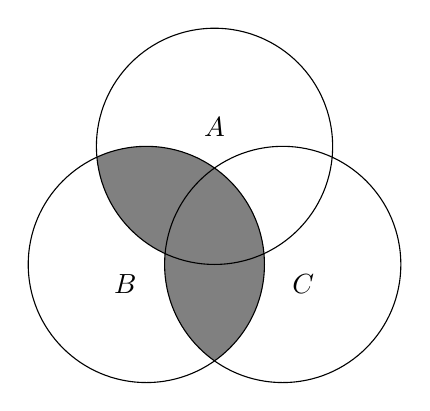
\begin{tikzpicture}
      \begin{scope}
    \clip \firstcircle;
    \fill[gray] \secondcircle;
      \end{scope}
      \begin{scope}
    \clip \secondcircle;
    \fill[gray] \thirdcircle;
      \end{scope}
      \draw \firstcircle node[text=black,above] {$A$};
      \draw \secondcircle node [text=black,below left] {$B$};
      \draw \thirdcircle node [text=black,below right] {$C$};
    \end{tikzpicture}
\label{fig:venn}
\caption{A state is represented by Boolean values over the regions of a Venn diagram, corresponding to the presence or absence of unique object types.}
\end{figure}


This kind of situation model, in which only the unique object types are represented, can also be displayed as a Venn diagram (Figure 1).
%Syllogisms are arguments that relate two terms (denoted \emph{A} and \emph{C}) via a third term (\emph{B}). 
%The model is based on an ontology of situations represented by Venn diagrams corresponding to all possible logical relations between the sets of three properties: A, B, C. 
%The choice of explicit representation of object~vs.~object types
The Venn diagram contains eight regions $i \in R$, corresponding to the unique object types that could be referred to in the syllogism. 
Each region corresponds to the presence or absence of each of the three properties: $\{\{A,B,C\},$ $\{A,B,\neg C\},$ $\{A,\neg B,C\},$ $\{\neg A, B, C\},$ $\{A, \neg B, \neg C\},...\}$. (For simplicity, when possible, we will refer to regions by the properties that are present, omitting the absent properties; for example, $\{A, B, \neg C\}$ will be referred to as $AB$.)
%These regions can be thought of as unique object types (e.g., an object defined by having properties $A$ and $B$ but not $C$) that are present in a situation.\footnote{This diagram representation is analogous to a mental model in the style of \citeA{johnson1983mental} composed of object tokens (e.g., some objects which have properties $A$ or $B$, etc.) but where only unique object tokens are represented (e.g., there cannot be two objects which have the same set of properties).}
Then, a state or situation (Venn diagram) $s \in S$ is composed of the set of object types (regions) that are present (e.g., $\{AB, BC, ABC\}$ is one possible state).
The set of unique states that we consider has size $2^7 = 128$.\footnote{
There are $2^7$ states and not $2^8$ states since the empty region (or, the object type which has neither of the three properties: $\{\neg A, \neg B, \neg C\}$) does not impact the truth conditions of the quantifier sentences used in syllogisms.
}
%, though we exclude the state where all eight regions are empty (i.e., the state where there are no As, Bs, and Cs, but also no things that are not As, Bs, or Cs).




%\subsection{Semantics}
The classical syllogisms are comprised by two premise arguments where each premise relates two properties via a quantifier. 
The quantifiers in classical syllogism are \emph{all}, \emph{some}, \emph{none}, and \emph{not all}.\footnote{
These quantifiers are typically presented in sentences such that \emph{none} is rendered as \emph{no} (e.g., No As are Bs) and \emph{not all} is rendered as \emph{some \_\_ are not} (e.g., Some As are not Bs).
}
We use the classic logical semantics of these quantifiers described in Table \ref{tab:sem}.
%\mht{CHECK THIS:
We assume the semantics of \emph{All As are Bs} describes a situation in which there exist objects that have the first property, sometimes referred to as the ``existential presupposition'' (e.g., \emph{All As are Bs} is false if there are no As, and hence \emph{All As are Bs} entails \emph{Some As are Bs}). 
%}
%: \emph{All As are Bs} entails that $\nexists (A \& \neg B)$;  \emph{Some As are Bs} entails that $\exists (A \& B)$; \emph{Some As are not Bs} entails that $\exists (A \& \neg B)$; \emph{No As are Bs} entails that $\nexists (A \& B)$.


% Please add the following required packages to your document preamble:
%\begin{table}[]
%\centering
%\begin{tabular}{@{}lll@{}}
%\toprule
%Example syllogistic sentence & Consistent State & Inconsistent state \\ \midrule
%All As are Bs                & \{AB, ABC\}      & \{A, ABC\}         \\
%Some As are Bs               & \{A, AB\}        & \{A, AC\}          \\
%Some As are not Bs           & \{A, AB\}        & \{AB, ABC\}        \\
%No As are Bs                 & \{A, AC\}        & \{A, AB\}          \\ \bottomrule
%\end{tabular}
%\caption{cap}
%\end{table}


% Please add the following required packages to your document preamble:
% \usepackage{booktabs}
\begin{table}[b]
\begin{tabular}{@{}llll@{}}
\toprule
Example syllogistic sentence & Logical Meaning                                                                       & Consistent State & Inconsistent state \\ \midrule
All As are Bs                                      & $\forall i \in R: A(i) \implies B(i) $ & \{AB, ABC\}                           & \{A, ABC\}                              \\
Some As are Bs                                     & $\exists i \in R: A(i) \implies B(i) $ & \{A, AB\}                             & \{A, AC\}                               \\
Some As are not Bs                                 & $\exists i \in R: A(i)  \centernot \implies B(i) $ & \{A, AB\}                             & \{AB, ABC\}                             \\
No As are Bs                                       & $\forall i \in R: A(i) \centernot \implies B(i) $  & \{A, AC\}                             & \{A, AB\} \\ \bottomrule
\end{tabular}
\caption{Logical meanings of example syllogistic sentences with examples of states that are consistent with the literal meanings and inconsistent with the literal meanings.}
\label{tab:sem}
\end{table}

\subsection{Interpreting the premises}
%\ndg{it'd be good to first say here that our model has a prior over these possible situations...}
%Our model \ndg{actually, consider moving this eqn down until after a need for prior is clear from the L0 model.}
%Given a representation of different states (Venn diagrams), 
We now introduce a probabilistic listener model that updates their beliefs about the states given the premises of the syllogism. 
The model's prior on states $P(s)$ is constructed by sampling a Bernoulli random variable for each of the $i \in R$ regions: $P(s) = \prod_{i \in R} P(A_{i}, B_{i}, C_{i})$. %= (P(a) \cdot P(b) \cdot P(c)) ^n$$
%This interpretation process can occur at the level of a literal listener (who updates beliefs based on the truth-conditional meaning of the premises) or a pragmatic listener who interprets the premises by reasoning about why a speaker chose to produce the premises that she did. 
%\subsubsection{Premise interpretation}
The premises of a syllogism update this prior on states via the literal, truth conditional meaning of each of the premises (shown in Table \ref{tab:sem}):
%All our recursive reasoning modeling components ground out in a model of literal interpretation.
%This model component is 
\begin{equation}
L_0(s \mid u ) \propto P(s)\cdot \mathcal{L}(u, s) 
\label{eq:L0}
\end{equation}
\noindent where $\mathcal{L}(u, s)$ is the lexicon that encodes the literal meanings of the quantified utterances used in syllogisms. 
These meanings can resolve to deterministic outcomes (e.g., $\mathcal{L}(u, s) = 1$ if the utterance $u$ is true of $s$, and 0 otherwise). 
In practice, however, we assume a small amount of noise $\phi$ in the semantics such that logically true $\mathcal{L}(u, s)$ may be judged false with probability proportional to $1-\phi$; conversely, states which are literally incompatible the utterance with have a small ($\phi$) probability of being judged true (rather than a 0 probability).
Equivalently, we assume a continuously valued semantics such that $\mathcal{L}(u, s) = 1-\phi$ or $\phi$, a technique introduced by \citeA{degen2020redundancy}.


The model of literal interpretation can be used to update the prior distribution on states (Venn diagrams) into a posterior distribution given the meaning of the premises of the syllogism. 
For the interpretation of a syllogism, $u$ is composed of two utterances (the two syllogistic premises): $u_1$ and $u_2$. 
Belief updating proceeds by assuming both utterances are true: 
\begin{equation}
L_0(s \mid u_1,  u_2) \propto P(s)\cdot \mathcal{L}(u_1, s) \cdot \mathcal{L}(u_2, s) 
\label{eq:L0premises}
\end{equation}


%\begin{figure*}[b]
%    \centering
%    \begin{subfigure}[t]{0.75\textwidth}
%        \centering
%        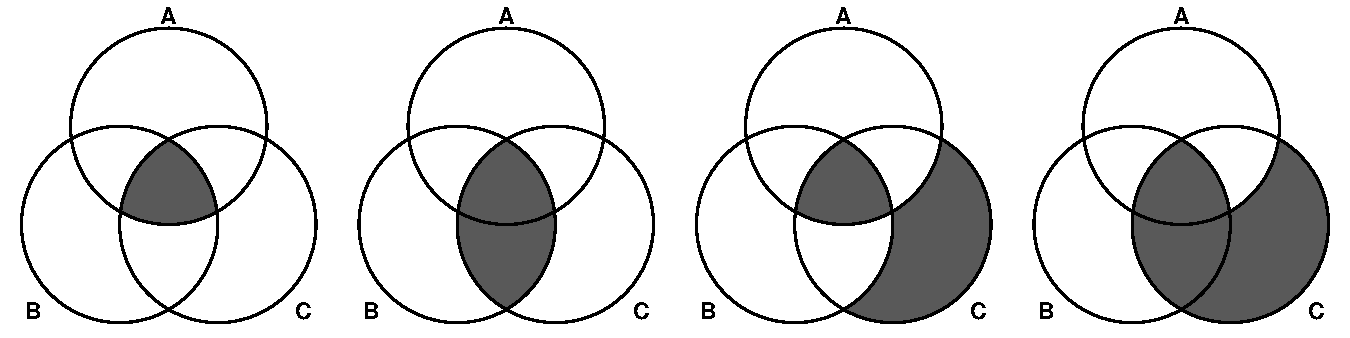
\includegraphics[width = 1\textwidth]{figs/diagrams_allAB_allBC.pdf}
%        \caption{Set of states literally compatible with the premises. The conclusion relation \emph{All As are Cs} is true in every compatible state.}
%    \end{subfigure}%
%    ~ 
%    \begin{subfigure}[t]{0.25\textwidth}
%        \centering
%        \includegraphics[width = 0.8\textwidth]{figs/venn_AA1_exp.pdf}
%        \caption{Literal interpreter's posterior expectation. }% over the regions of the Venn diagram implied by the premises.}
%    \end{subfigure}
%    \caption{States (Venn diagrams) implied by the logically valid syllogism: \emph{All As are Bs}, \emph{All Bs are Cs}. Opacity of region represents posterior probability.}
%\end{figure*}

\begin{figure}[b]
\centering
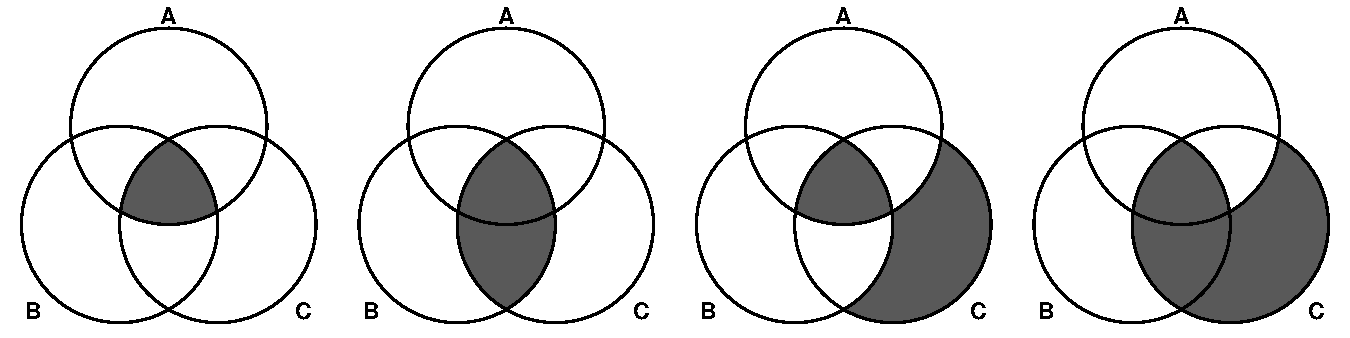
\includegraphics[width = \textwidth]{figs/diagrams_allAB_allBC.pdf}
\caption{Set of Venn diagrams (states) literally compatible with the premises of the logically valid syllogism: \emph{All As are Bs}, \emph{All Bs are Cs}. The conclusion relation \emph{All As are Cs} is true in every compatible state.}
\label{fig:AAvenns}
\end{figure}


Equation \ref{eq:L0premises} defines a probability distribution over states (Venn diagrams) given the premises of the syllogism. 
Logically valid syllogisms give rise to a distribution over states where a quantifier relationship between the conclusion terms of the syllogism is true in all possible states given the premises. 
For example, in the logically valid syllogism  \emph{All As are Bs}, \emph{All Bs are Cs} (the ``Barbara'' syllogism), the relationship \emph{All As are Cs} is true in every possible state in which the premises are true; in particular, the region \emph{ABC} (an object which has all three properties) is true in every possible state (Figure \ref{fig:AAvenns}).
On the other hand, the premises of logically invalid syllogisms tend to give rise to many possible states in which no particular syllogistic conclusion is true in every state; some conclusions are true in more states, however, than other conclusions.
For example, in the logically invalid \emph{No As are Bs}, \emph{Some Bs are Cs}, the conclusion \emph{All As are Cs} is logically possible though is true in fewer states than \emph{No As are Cs} (Figure \ref{fig:EIvenns}).


\begin{figure}[t]
\centering
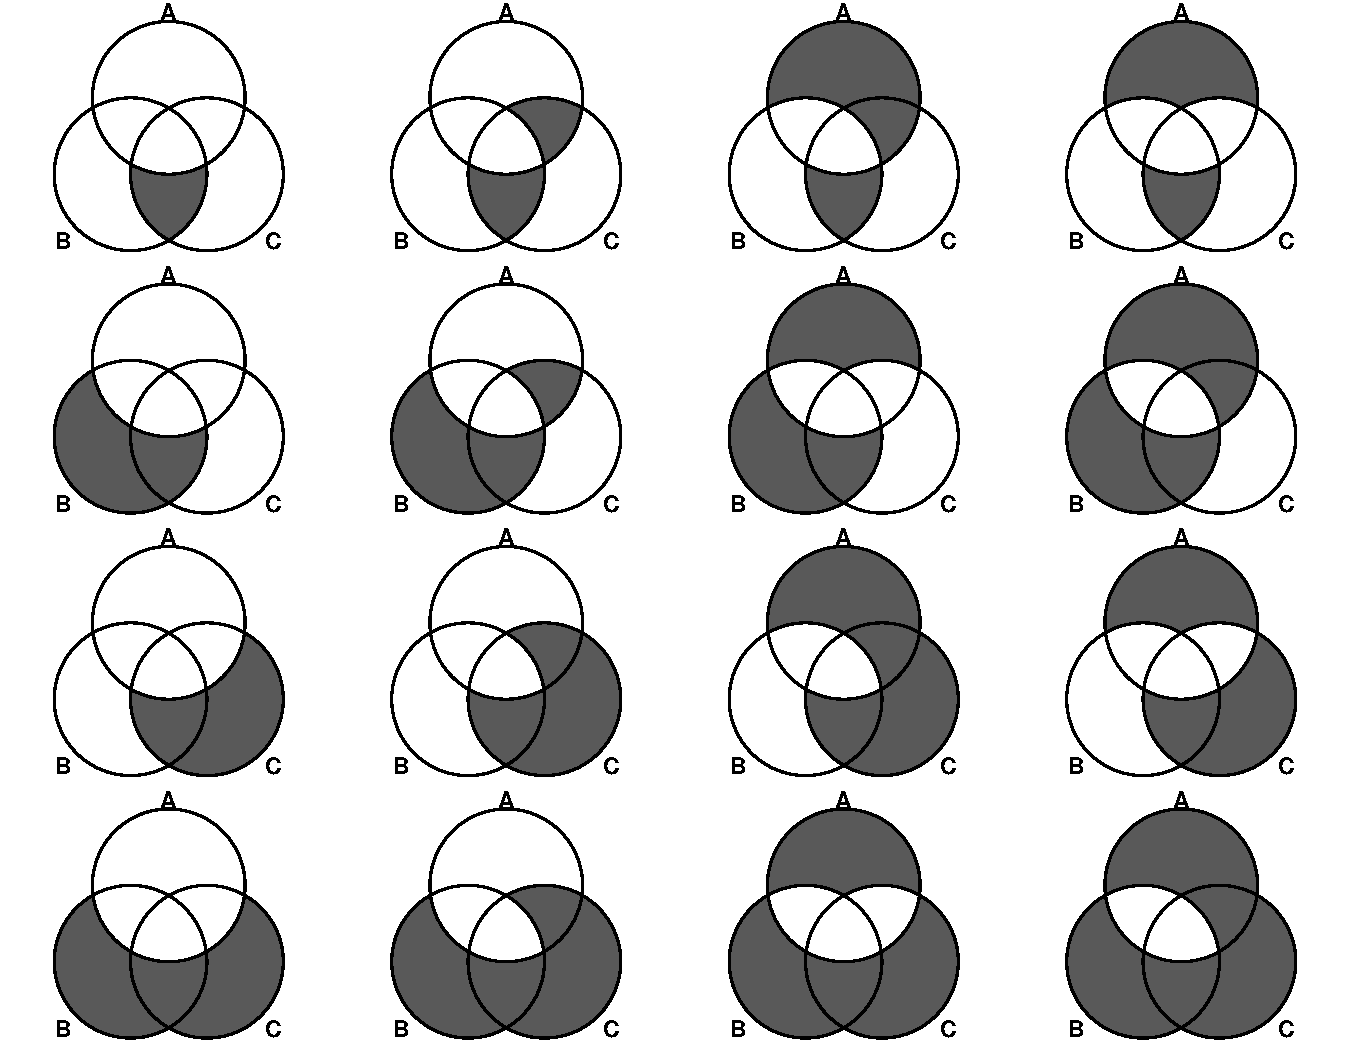
\includegraphics[width = \textwidth]{figs/diagrams_noneAB_someBC.pdf}
\caption{Set of Venn diagrams (states) literally compatible with the premises of the logically invalid syllogism: \emph{No As are Bs}, \emph{Some Bs are Cs}. No syllogistic conclusion is true in every compatible state.}
\label{fig:EIvenns}
\end{figure}


%\begin{figure*}[t]
%    \centering
%    \begin{subfigure}[t]{0.75\textwidth}
%        \centering
%        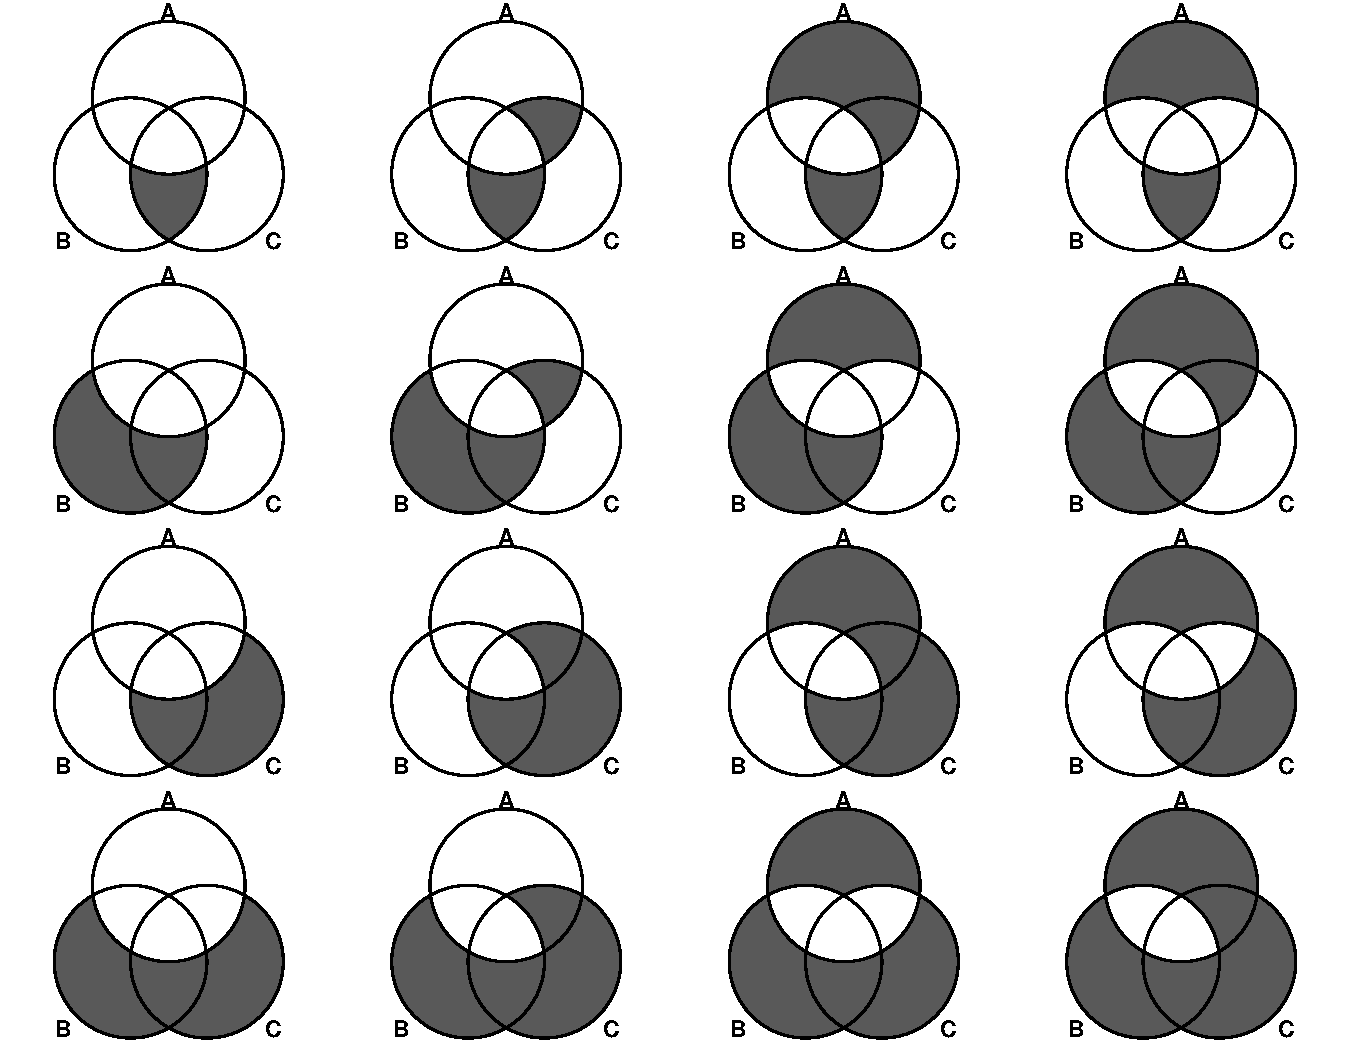
\includegraphics[width = 1\textwidth]{figs/diagrams_noneAB_someBC.pdf}
%        \caption{Set of states literally compatible with the premises. No syllogistic conclusion is true in every compatible state.}
%    \end{subfigure}%
%    ~ 
%    \begin{subfigure}[t]{0.25\textwidth}
%        \centering
%        \includegraphics[width = 0.8\textwidth]{figs/venn_EI1_exp.pdf}
%        \caption{Literal interpreter's posterior expectation. }% over the regions of the Venn diagram implied by the premises.}
%    \end{subfigure}
%    \caption{States (Venn diagrams) implied by the logically invalid syllogism: \emph{No As are Bs}, \emph{Some Bs are Cs}. Opacity of region represents posterior probability.}
%    \label{fig:EIvenns}
%\end{figure*}

%\begin{figure}[t]
%\centering
%\includegraphics[width = \textwidth]{figs/venn_literal_AA1_AI1_EI1_exp_wQUD.pdf}
%\caption{Literal interpreter model's posterior expectation over the regions of the (i) full state (Venn diagram) and (ii) Question Under Discussion (A-C) implied by three syllogisms. Darker opacity denotes higher posterior probability.}
%\label{fig:EIvenns}
%\end{figure}


%\begin{figure*}[b]
%    \centering
%    \begin{subfigure}[t]{\textwidth}
%        \centering
%        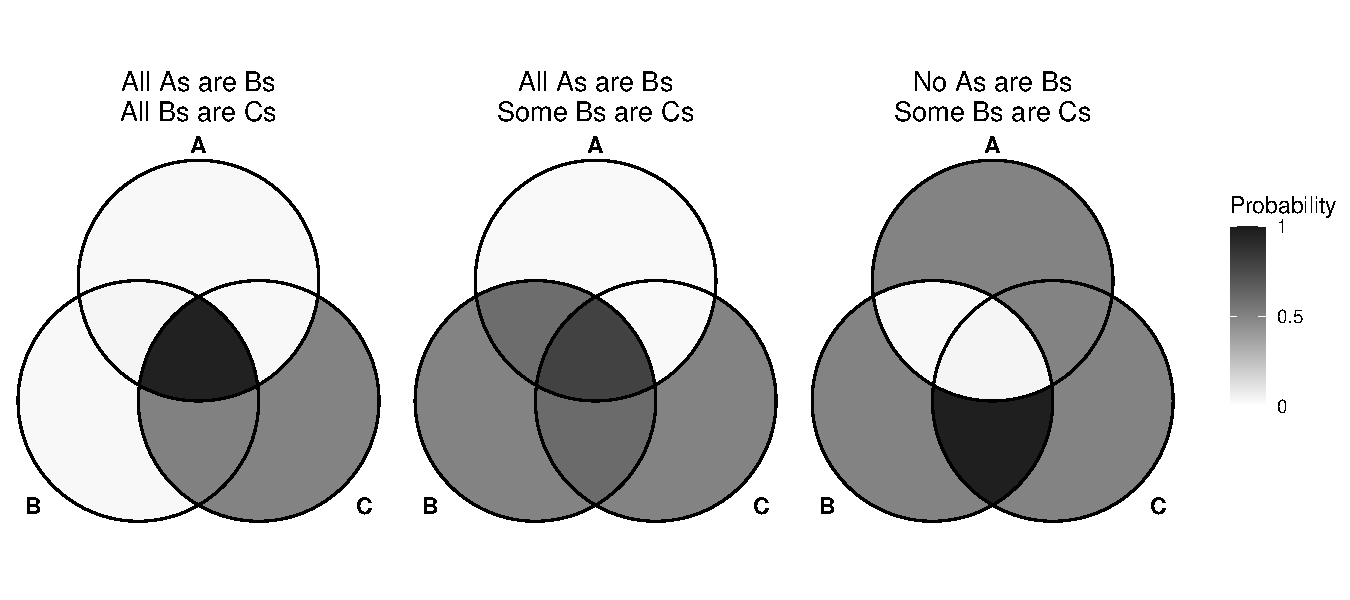
\includegraphics[width = 0.85\textwidth]{figs/venn_literal_AA1_AI1_EI1_exp.pdf}
%%        \caption{Set of states literally compatible with the premises. The conclusion relation \emph{All As are Cs} is true in every compatible state.}
%    \end{subfigure}
%    
%    \begin{subfigure}[t]{\textwidth}
%        \centering
%        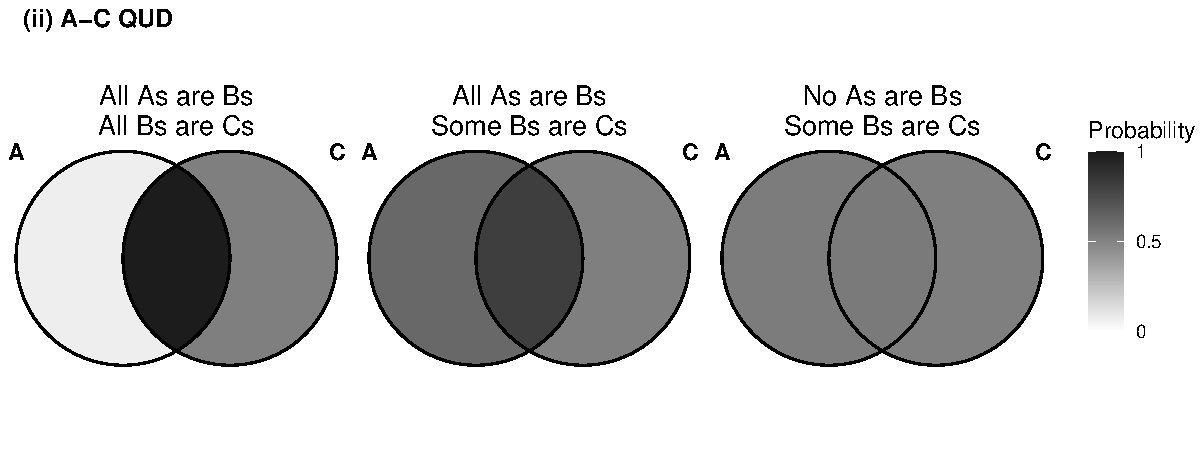
\includegraphics[width = 0.85\textwidth]{figs/venn_literal_AA1_AI1_EI1_exp_qud.pdf}
%%        \caption{Literal interpreter's posterior expectation. }% over the regions of the Venn diagram implied by the premises.}
%    \end{subfigure}
%    \caption{\small Literal interpreter model's posterior expectation over the regions of the (i) Full State (Venn diagram) and (ii) Question Under Discussion (A-C) implied by three syllogisms. The A-C Question Under Discussion reduces the dimensionality of the state and blurs distinctions between different Venn diagrams. Darker opacity denotes higher posterior probability.}
%    \label{fig:lit_state_qud}
%\end{figure*}


\begin{figure}[b]
    \centering
        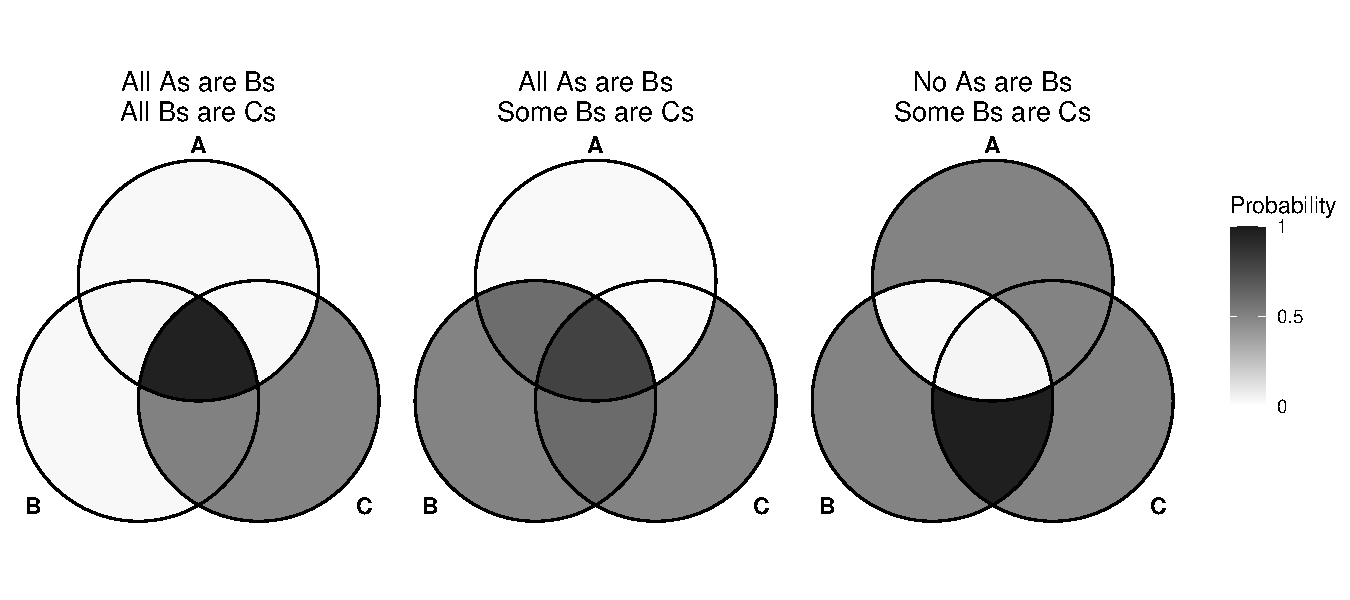
\includegraphics[width = 0.95\textwidth]{figs/venn_literal_AA1_AI1_EI1_exp.pdf}
    \caption{ Literal interpreter model's posterior expectation over each of the regions of the state implied by three syllogisms. Darker opacity denotes higher posterior probability.}
    \label{fig:lit_state_qud}
\end{figure}







\subsection{Producing a conclusion}

The second component of a syllogistic reasoning model is a model of conclusion production. 
That is, given a set of beliefs about the likely state of affairs (Eq.~\ref{eq:L0premises}), what conclusion should be drawn?
We formalize three models of conclusion production.
The first is a literal speaker, who selects conclusions that are true given the speaker's beliefs about the state. 
The second is a pragmatic speaker, who selects a conclusion that would best convey information about an individual likely state to a naive listener (\emph{State communication}). 
Our third and most sophisticated model is of a pragmatic speaker who chooses utterance to convey information about her entire belief distribution over states (\emph{Belief alignment}). 
%align a naive listener's beliefs about the state with the beliefs of the speaker.
%Since these models produce a distribution over conclusions, we label these models as reasoner models $R$, so as to not confuse them with the speaker models $S$ that are used as part of the recursion in the pragmatic interpretation of premises. \mht{switch to $S$ since no more pragmatic interpretation?}
%The pragmatic production of a conclusion is a model of a speaker who tries to produce the most informative utterance (conclusion) to convey information to a naive listener. 

\subsubsection{Space of conclusions}

The syllogistic reasoning task presents participants with a set of options for the quantifier relationship between the two terms of the syllogisms that are not described explicitly in relation to each other in the premises (i.e., the terms \emph{A} and \emph{C} if the premises are of the form \emph{A -- B}, \emph{B -- C}.). 
Particular tasks differ in the set of options that are given to participants, but the maximal set includes the four quantifiers  (\emph{all}, \emph{some}, \emph{not all}, \emph{none}) crossed with the two orderings of the terms of the conclusion (i.e., \emph{A -- C} or \emph{C -- A}).
Thus, there are eight quantified conclusion options. 

A ninth unique option, however, is also available: the option that \emph{nothing follows} (sometimes described \emph{no valid conclusion}). 
The \emph{nothing follows} conclusion is the logically correct answer for the logically invalid syllogisms and is produced to variable extents by participants in both logically valid and invalid syllogisms \cite{Khemlani2012}.
While the semantics of the quantifier conclusions are quite clear (Table \ref{tab:sem}), the proper treatment of the \emph{nothing follows} conclusion is not obvious. 
Extant theories treat this option indirectly, either as a byproduct or last resort of a reasoning process, when it is treated at all \cite{ragni2019does, riesterer2020modeling}.
We approach the question of the meaning of \emph{nothing follows} from a language production standpoint, where we formalize the statement as tantamount to not saying anything at all. 
Formally, we model the \emph{nothing follows} statement as a vacuous, or silent, utterance: an utterance which is true in every possible state of affairs.
Hence, the impact of using such an utterance is that it does not serve to update a listener's beliefs about the state. 
% From a language production perspective, however, the


\subsubsection{Literal production of conclusions}

% In a classical reasoning model, these 
% lexical meanings such that
% Our pragmatics model begins with submodal that performs a literal interpretation of the premises. 
% The model computes a 
Given a belief updating model based on the premises of a syllogism $L_0$, %(either literal $L_0$ or pragmatic $L_1$), 
we define a literal production model $S_0$ that uses the listener $L_0$'s posterior distribution on states to determine what conclusion is likely to be true given the premises. 
This model $S_0$ can be viewed as one that is sampling a state from the listener's posterior distribution on states and randomly selecting among the conclusions that are literally true of that state. 

%The strength of a syllogistic argument (two premises) for a conclusion is a real-valued number between 0 and 1 given by the $P(u_c \mid u_1, u_2)$, where $u_1$ and $u_2$ are the two premises of the syllogism.

\begin{equation}
S_0(u_3 \mid u_1, u_2) \propto \sum_s \mathcal{L}(u_3, s) \cdot L_0(s \mid u_1, u_2) \label{eq:R0}
\end{equation}

\subsubsection{Informative production of conclusions: State communication}

We define a more sophisticated speaker model who selects conclusions in order to convey information to a naive listener (who has heard neither premises nor conclusion). 
Since the reasoner does not know the state (but only has beliefs about the state given the premises of the syllogism), we operationalize the informational utility of a conclusion by marginalizing over the speaker's beliefs about the state.
This speaker model first samples a state from the conditional distribution on states given the premises (as did the literal speaker in Eq.~\ref{eq:R0}).
Following standard practice in the Rational Speech Act modeling framework, the utility of the utterance for a particular state is the negative surprisal of the state given the utterance.
The speaker then chooses utterances soft-max optimally with respect that utility function.

\begin{equation}
S_1(u_3 \mid u_1, u_2) \propto \exp{ [ \alpha \cdot  \sum_s  \ln L_0(s \mid u_3) \cdot L_0(s \mid u_1, u_2) ] } \label{eq:R1a}
\end{equation}

Note that the two $L_0$'s in Eq.~\ref{eq:R1a} are actually two different agents.
$L(s \mid u_1, u_2)$ is the reasoner who updates their beliefs about the state given the premises.
$L(s \mid u_3)$ is a hypothetical listener that the reasoner is communicating with; they update their beliefs about the state from the conclusion ($u_3$).
The priors and likelihoods of these agents are equivalent and thus are represented equivalently. 
%\ndg{add a note that the two L0's in this eqn are actually the two different agents, but they are treated equivalently?}

% \mht{this sampling a state idea might be directly analogous to how mental models theory treats this conclusion selection process (with respect to a particular model)...}

\subsubsection{Informative production of conclusions: Belief alignment}

Rather than the speaker sampling a state and then selecting an utterance to describe that state, the informational utility can be defined with respect to the reasoner's full belief distribution over states \cite{Goodman2013, scontras2018probabilistic}. 
The utility of a conclusion, then, is quantified by how well it would align the listener's beliefs with those of the reasoner. 
Formally, we use the information-theoretic measure of Kullback-Leibler (KL) divergence as the measure of alignment of the naive listener and reasoner's belief distributions. 
%Again, this formalization is agnostic as to how we compute the reasoner's state distribution (whether it be via a literal or a pragmatic interpretation of the premises), and so 
We denote the reasoner's belief distribution over the state as $S= L_0(s \mid  u_1,u_2)$. 

\begin{align}
  \label{eq:KL-divergence}
  \text{KL}({ S \mid \mid L_0}(u)) = \sum_{s}  S(s) \ \log \frac{ S(s)}{{L_{0}}(s \mid u)}
\end{align}

\noindent Then, the speaker model that selects conclusions an informative manner is given by: 

\begin{equation}
S_1(u_3 \mid u_1,  u_2) \propto  \exp [ \alpha_2 \cdot - \text{KL}({ L_0(s \mid  u_1,u_2) \mid \mid L_0}(s \mid u_3)) ]  \label{eq:R1b}
\end{equation}

\noindent where $L_0(s \mid u)$ is the literal listener model defined in Equation \ref{eq:L0}. 

We note that a critical ingredient to this Belief Alignment model of conclusion production is the noisy semantics we assume inside the literal listener $L_0$.
Without it, the speaker would be required to say \emph{nothing follows} for any logically invalid syllogism. 
A logically invalid syllogism is one in which no conclusion is true in every state in which the premises are true.
If a speaker were to choose one of these conclusions, then the states that are incompatible with the conclusion would be imagined (by the listener) to have 0 probability. 
But since the conclusion is not logically valid, the speaker believes these states to have non-zero probability.
This combination leads Eq.~\ref{eq:KL-divergence} to be undefined, which results in the model always saying \emph{nothing follows} for logically invalid syllogisms.
By adding a small amount of noise into the semantics, we avoid this boundary case.


%If there is not a conclusion which is always true, then the states which make the conclusions false have non-zero probability. 
%
%The reason for this degenerate behavior is that any quantifier conclusion will deterministically rule out certain states (i.e., set their probability equal to 0). 
%Thus, for a logically invalid syllogism,  there exists no set of states that support the truth of a particular quantifier
%
%
%
%producing a quantified conclusion, the speaker would be conveying that a certain state has 0 probability, when in the mind of the speaker, the state has non-0 probability. 

%Hearing any quantified statement; thus, the speaker's belief distribution will ascribe probability 0 to certain states.
%Hearing \emph{nothing follows} rules out no states; thus, the naive listener's belief distribution will have no states with probability 0.

%actually, i think i got the 3rd point in reverse: the issue is that the speaker will only say “nothing follows” (for all logically invalid syllogisms) in order to avoid ruling out states that have non-zero probability

%Then, the utility of \emph{nothing follows} in terms of the KL-distance between the speaker and listener's belief distributions 
%A speaker would 
%
% be infinitely bad because it will imply some states have non-zero probability when in fact they have zero probability (according to the premises)

%prior distribution over situations with the literal meanings of the quantified statements: 


%Using KL-divergence, we can then state a more general definition of utterance utilities, to
%replace \eqref{U}:
%\begin{align}
%  \label{eq:Utils-KL-based}
%  U_{S_1}(u; s) = \text{KL}(P_{S_{1}\text{-}Bel} \mid \mid P_{L_{0}\text{-}Bel}(u)) - C(u)
%\end{align}


\section{Modeling the Ragni et al. (2019) data set}

We test our models using a dataset published by \citeA{ragni2019does}. 
The data set consists of the results of a web experiment in which participants ($n = 139$) provided conclusions to all 64 syllogisms. In the experiment, participants completed all syllogistic reasoning problems after a brief training phase. Participants responded by selecting one of the nine possible responses for the conclusion of the syllogism (4 quantifier choices x 2 term orders + 1 \emph{nothing follows}). 
%\ndg{perhaps say why we use this dataset instead of the many others?}
We use this data set because it is large and comprehensive (i.e., has many responses for all 64 syllogisms). 
%Participants' responses to four example syllogisms are shown in Figure \ref{fig:ragniData}).

%\begin{figure}[th]
%\centering
%\includegraphics[width = \textwidth]{figs/ragni_4sylls.pdf}
%\caption{Human conclusion choices for four syllogistic reasoning problems from the \citeA{ragni2019does} data set.}
%\label{fig:ragniData}
%\end{figure}

%\subsection{Model space}
%
%We consider a space of three possible Rational Speech Act models of syllogistic reasoning, which vary in how they produce conclusions. 
%Premises could be interpreted literally (Eq.~\ref{eq:L0}), pragmatically with respect to a full state (Venn diagram) QUD (Eq.~\ref{eq:L1}), or pragmatically with respect to a Question Under Discussion that focuses on the relationship between the conclusion terms of the syllogism (Eq.~\ref{eq:L1q}).
%Conclusions can be produced either literally (Eq.~\ref{eq:R0}) or informatively (Eq.~\ref{eq:R1}).


\subsection{Bayesian data analysis}

To assess how well our models can accommodate the syllogistic reasoning data from \citeA{ragni2019does}, we embed each model variant (literal speaker, state communication, belief alignment) within a Bayesian data analysis model to infer the credible values of the latent parameters of the models and generate predictions given those parameters. 

\subsubsection{Parameters and priors}

The Rational Speech Act modeling framework assumes speakers are approximately rational agents who produce utterances as actions whose utility is defined by conveying information to a listener. The degree of rationality of the speaker interpolates between probability matching behavior and utility maximizing behavior. 
For these parameters, we assume uniform priors over the range of (0, 20), consistent with the prior literature on RSA models. 
We additionally assume a small amount of noise in the literal semantics of the utterances such that with a small probability $\phi$, the literal listener disregards the utterance heard and does not update its beliefs via that utterance; we put a uniform prior over the limited range of (0, 0.1) over this parameter since we assume the noise to be a small quantity. 
For simplicity, we parametrize the prior distribution over states $P(x)$ in the reasoner models in a strictly uninformative manner: all regions (object types) have equal probability of being true, which is fixed to 0.5.\footnote{
We experimented with more flexible parameterizations of the prior but found that these did not significantly improve model performance on this data set.}

% via independent Bernoulli random variables $\theta_k$ corresponding to the prior probability of each of the seven regions of a Venn diagram; we put uniform priors over the unit interval for these parameters.

Finally, we assume one global ``irrationality'' parameter that modulates the pragmatic reasoner's prior preferences for conclusions with a specific ordering of the terms (A--C vs. C--A) based on the ordering of the terms in the premises. 
These preferences are sometimes referred to as ``figural effects'', tracing back to the ``figure'', or term orderings, of the premises \cite{Wetherick1990, rips1994}.
Our goal is not to provide an explanation for these effects, but rather posit an effect in line with the observations of \citeA{JL1984, JL1978, geurts2003reasoning} that participants prefer conclusions whose subject term matches the subject of one of the premises.
Formally, the conclusion prior is parameterized by unnormalized probability weights, where a uniform prior would have a weight of 1 for all conclusions. 
% The first parameter is a global preference or dispreference $\beta_0$ for the \emph{nothing follows} conclusion; we put a uniform prior between (0, 2) on this weight. 
We introduce a global preference  parameter $\beta$ for conclusions whose order of the terms (A--C vs. C--A) matches the order of the terms in the premises.
This first-term preference works by checking whether either A or C appear in the subject position of one of the premises.
If only one appears in the subject (e.g., the syllogistic frame \emph{A--B/B--C}), then conclusions where that same term appears in the subject (e.g., \emph{A--C}) will have a prior preference determined by $\beta$.
If both or neither appear in the subject (e.g., \emph{A--B/C--B} or \emph{B--A/B--C}), then no preference is given in the conclusion prior, corresponding to an unnormalized probability weight of 1. 
We put a uniform prior between (1, 5) on this preference weight since we assume it to be preference for producing conclusions that match the order of the terms of the syllogism. 





%In our model, we have two speaker components: one involved in the pragmatic interpretation of the premises and one involved in the pragmatic production of conclusions; each of these carries with a speaker optimality parameter $\alpha$. 


\begin{figure}[ht!]
\begin{center}
\begin{tabular}{cc}
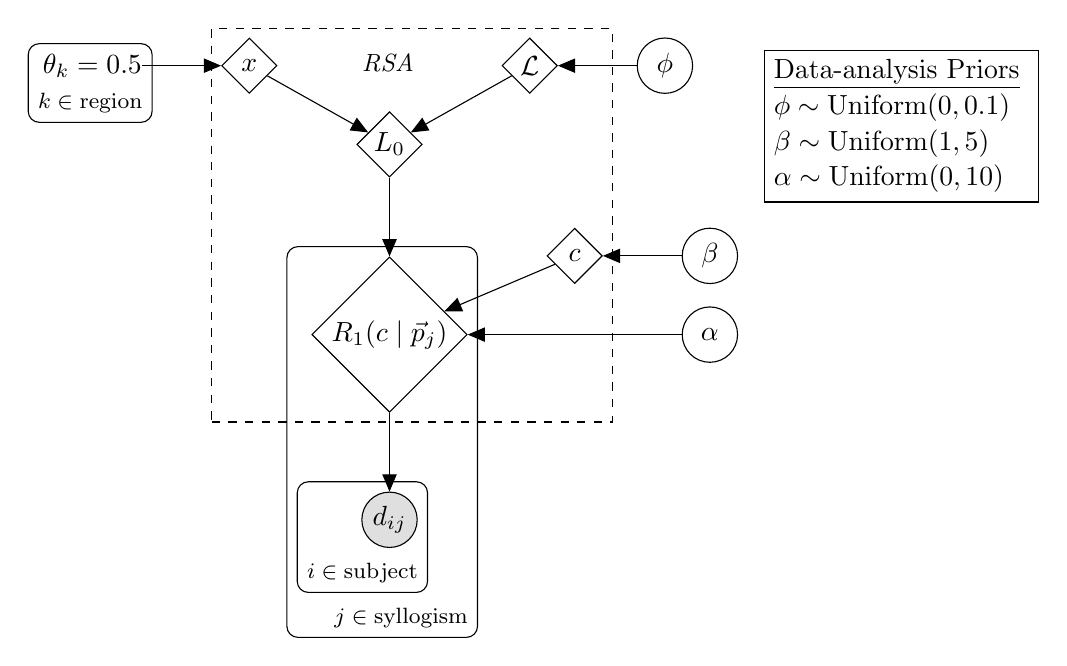
\begin{tikzpicture}
%% RSA nodes and data
\node[obs](data){$d_{ij}$};

\node[det, above=of data](R1){$R_{1}(c \mid \vec{p}_j)$};
\node[det, above=of R1](L0){$L_{0}$};

\node[det, left=of L0, yshift=1cm](x){$x$};
\node[const, left=of x](theta){$\theta_k = 0.5$};

\node[det, right=of L0, yshift=1cm](lex){$\mathcal{L}$};
\node[latent, right=of lex](phi){$\phi$};

\node[det, right=of R1, yshift=1cm](c){$c$};
\node[latent, right=of c](b0){$\beta$};

\node[latent, right=of c, yshift=-1cm](alpha2){$\alpha$};

\gate {RSAgate} {(R1)(L0)(lex)(x)(c)} {} ; %

\plate{plate_region}{(theta)}{$k \in \text{region}$};
\plate{plate_data}{(data)}{$i \in \text{subject}$};

\plate{plate_syllogism}{
 (R1)(data)(plate_data)
}{$j \in \text{syllogism}$}


\edge{R1}{data};
\edge{L0}{R1};
%\edge{S1}{L1};
%\edge{L0}{S1};

\edge{theta}{x};

\edge{x}{L0};
%\edge{x}{L1};

\edge{lex}{L0};
\edge{phi}{lex};

%\edge{alpha1}{S1};

\edge{c}{R1};
\edge{b0}{c};

\edge{alpha2}{R1};

\node[text width=1cm] at (0.15,5.8) {\emph{\small{RSA}}};

\node[draw, align=left, execute at begin node=\setlength{\baselineskip}{3ex}] at (6.5, 5) { 
\text{\underline{Data-analysis Priors} } \\ 
%$ \theta_k  \sim \text{Uniform}(0, 1)$ \\
$ \phi  \sim \text{Uniform}(0, 0.1)$ \\
$ \beta  \sim \text{Uniform}(1, 5)$ \\
$ \alpha \sim \text{Uniform}(0, 10)$ 
};


%\begin{figure}[ht!]
%\begin{center}
%\begin{tabular}{cc}
%\begin{tikzpicture}
%%% RSA nodes and data
%\node[obs](data){$d_{ij}$};
%
%\node[det, above=of data](R1){$R_{1}(c \mid \vec{p}_j)$};
%\node[det, above=of R1](L1){$L_{1}$};
%\node[det, above=of L1](S1){$S_{1}$};
%\node[det, above=of S1](L0){$L_{0}$};
%
%\node[latent, left=of S1](x){$x$};
%\node[latent, left=of x](theta){$\theta_k$};
%
%\node[latent, right=of L0](lex){$\mathcal{L}$};
%\node[latent, right=of lex](phi){$\phi$};
%
%\node[latent, right=of S1, xshift=1.74cm](alpha1){$\alpha_1$};
%
%\node[latent, right=of L1](c){$c$};
%\node[latent, right=of c, yshift = 0.5cm](b0){$\beta_0$};
%\node[latent, right=of c, yshift = -0.5cm](b1){$\beta_1$};
%
%\node[latent, right=of R1, xshift=1.2cm](alpha2){$\alpha_2$};
%
%\gate {RSAgate} {(R1)(L1)(S1)(L0)(lex)(x)(c)} {} ; %
%
%\plate{plate_region}{(theta)}{$k \in \text{region}$};
%\plate{plate_data}{(data)}{$i \in \text{subject}$};
%
%\plate{plate_syllogism}{
% (R1)(data)(plate_data)
%}{$j \in \text{syllogism}$}
%
%
%\edge{R1}{data};
%\edge{L1}{R1};
%\edge{S1}{L1};
%\edge{L0}{S1};
%
%\edge{theta}{x};
%
%\edge{x}{L0};
%\edge{x}{L1};
%
%\edge{lex}{L0};
%\edge{phi}{lex};
%
%\edge{alpha1}{S1};
%
%\edge{c}{R1};
%\edge{b0}{c};
%\edge{b1}{c};
%
%\edge{alpha2}{R1};
%
%\node[text width=1cm] at (-1.65,8.65) {\emph{\small{RSA}}};
%
%\node[draw, align=left, execute at begin node=\setlength{\baselineskip}{3ex}] at (6.5, 7.5) { 
%\text{\underline{Data-analysis Priors} } \\ 
%$ \theta_k  \sim \text{Uniform}(0, 1)$ \\
%$ \phi  \sim \text{Uniform}(0, 0.1)$ \\
%$ \beta_0  \sim \text{Uniform}(0, 2)$ \\
%$ \beta_1  \sim \text{Uniform}(1, 5)$ \\
%$ \alpha_{1, 2}  \sim \text{Uniform}(0, 20)$ 
%};

%$\beta^\rho_0 ,\beta^\rho_1 \sim \text{Uniform}(-2,2)$ \\
% $\rho_i = \text{logistic}(\beta^\rho_0  + i \cdot \beta^\alpha_1)$ \\
% $d^{CG}_{i} \sim \text{Bernoulli}(\rho_i)$ \\
% \\
%$\beta^\alpha_0 \sim \text{Uniform}(-3,3); \beta^\alpha_1 \sim \text{Uniform}(-0,4)$ \\
% $\alpha_i = \beta^\alpha_0  + i \cdot \beta^\alpha_1$ \\
% \\
% $\mu^\theta_0 \sim \text{Uniform}(-3,3); \mu^\theta_1 \sim \text{Uniform}(0,2)$ \\
% $\sigma^\theta_0 \sim \text{Uniform}(0,2); \sigma^\theta_1 \sim \text{Uniform}(0,1)$ \\
% $\beta^\theta_0 \sim \text{Gaussian}(\mu^\theta_0, \mu^\sigma_0); \beta^\theta_1 \sim \text{Gaussian}(\mu^\theta_1, \mu^\sigma_1)$  \\
% $\theta_{ij} = \text{logistic}(\beta^\theta_{0,j}  + i \cdot \beta^\theta_{1,j})$ \\
% $d^{ME}_{ij} \sim L'_{ij},  d^{CM}_{ij} \sim L_{ijk}$
%};
%
%\node[draw, align=left, execute at begin node=\setlength{\baselineskip}{3ex}] at (8,0) {Integration model\\ $P_{L_{1}}(r \mid u; \{\rho_i, \alpha_i\, \theta_{ij}\})\propto P_{S}(u \mid r; \{\alpha_i, \theta_{ij}\}) \cdot P(r \mid \rho_i) $\\ 
%$P_{S}(u \mid r; \{\alpha_i\, \theta_{ij}\})\propto P(r \mid u; \{\theta_{ij}\}) ^{\alpha_i} $\\
%$P(r \mid u; \{\theta_{ij}\}) \propto \mathcal{L}(u, r \mid \theta_{ij})$
%};


\end{tikzpicture}

    \end{tabular}
  \end{center}
  \caption{\small Bayesian data analysis model. The conclusion choices for each $i$ participant on each $j$ syllogism $d_{ij}$ are generated via the pragmatic reasoner model $R_1$, which defines a conditional distribution on conclusions $c$ given premises $\vec{p}_j$. The reasoner model $R_1$ is a Rational Speech-Act (RSA) model that interprets premises according to a literal listener model $L_0$, which updates its beliefs according to the literal meaning $\mathcal{L}$ of the sentences it hears. Literal meanings are the standard, truth-functional meanings of the quantifiers (Table 1\label{tab:sem}) with a small amount of noise $\phi$. The prior distribution over states $P(x)$ is parameterized by independent Bernoulli weights $\theta_k$ for each of the 7 $k$ regions of a Venn diagram, which we assume are all equal to 0.5. The reasoner $R_1$'s prior distribution over conclusions includes a preference $\beta$ for term-orderings (A--C vs. C--A) that match the ordering of the terms in the premises. Finally, the reasoner $R_1$ that selects conclusions has a soft-max parameter $\alpha$.}
  \label{fig:bayesnet}
\end{figure}

\subsubsection{Implementation and inference}

We implemented the cognitive models and the Bayesian data analytic models in the probabilistic programming language WebPPL \cite{dippl}. 
To learn about the credible values of the parameters, we ran 3 MCMC chains each for 15,000 iterations discarding the first 5,000 iterations for burn-in. 
We assessed convergence through visual comparison of the posterior distributions to ensure that the inferences that resulted from looking at different chains were not appreciably different.
We performed model comparison by computing Bayes Factors, which quantify the likelihood of the data under each model averaging over the model's prior distribution over parameters. By averaging over each model's prior on parameters, Bayes Factors implicitly penalize models with extra degrees of freedom \cite{lee2014bayesian}.
We estimated the marginal likelihoods of the data under each model using an Annealed Importance Sampling algorithm \cite{neal2001annealed}.

\subsubsection{Results}

Overall, we found that the Belief Alignment pragmatic speaker model was the best fitting and most parsimonious model of the syllogistic reasoning data set. 
This model performed several orders of magnitude better at explaining the data, taking into the account model complexity (in comparison to the Literal Speaker model, $\log BF \approx 300$; in comparison to the State Communication pragmatic speaker $\log BF \approx 1200$).
It also achieved the highest correlation coefficient and lowest mean squared error of the RSA model variants (Table \ref{tab:altStats}).

\begin{figure}[t]
\centering
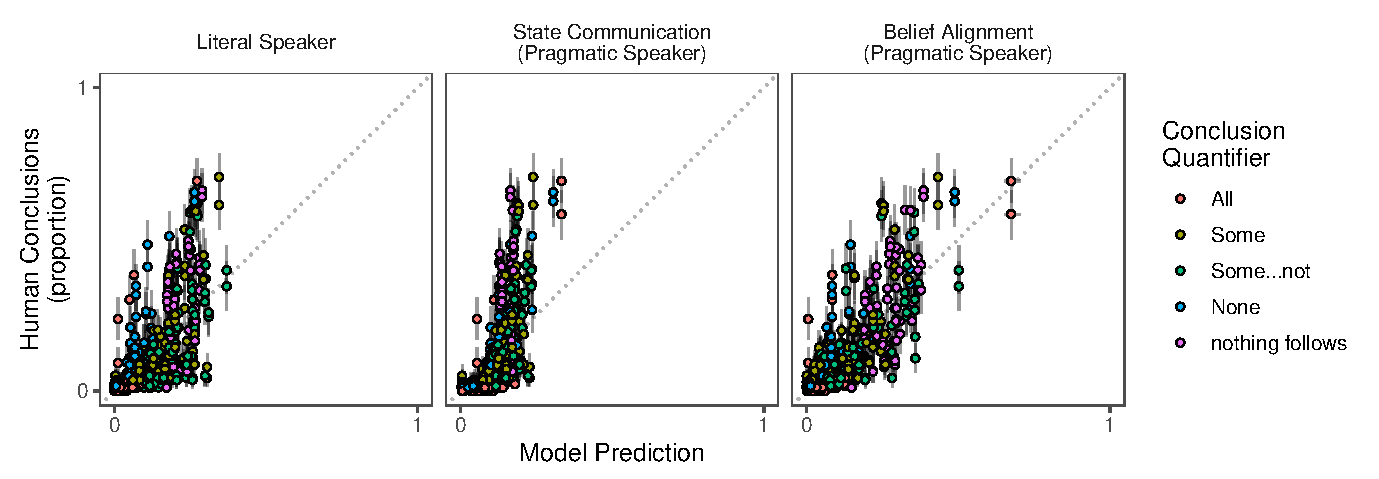
\includegraphics[width = \textwidth]{figs/bda_rsa_scatters_0paramPrior.pdf}
\caption{Posterior predictive model fits for the literal speaker model and two versions of the pragmatic speaker model. Each dot represents one of nine possible conclusions for one of the 64 possible syllogisms. Error bars denote bootstrapped 95\% confidence intervals for the empirical data and 95\% Bayesian credible intervals for the model predictions.}
\label{fig:scatters}
\end{figure}

The Belief Alignment Pragmatic Speaker model captures a number of interesting patterns in human syllogistic reasoning behavior. 
By incorporating a notion of informativeness into the selection of a conclusion, the model is able to  show a preference among equally true conclusions. For example, in the \emph{All As are Bs / All Bs are Cs} syllogism, the conclusion \emph{Some As are Cs} is true in every possible world that \emph{All As are Cs} is true, because \emph{all} entails \emph{some}. Nonetheless, the Belief Alignment pragmatic speaker model and human participants strongly prefer the \emph{all} conclusion (Figure \ref{fig:bars}, top-left facet); the model arrives at this preference because \emph{all} more informatively conveys the belief state of the speaker in comparison to \emph{some}.
%The model can also 

Syllogisms for which the premises provide little information about the conclusion also reveal interesting reasoning patterns in both participants and the models.
In the \emph{No As are Bs / No Bs are Cs} syllogism, participants tend to respond either \emph{nothing follows} (the logically correct conclusion) or either \emph{No As are Cs} or \emph{No Cs are As} (Figure \ref{fig:bars}, second row, second column). 
The Literal Speaker model reveals what is likely to be true given the premises: \emph{Some As are not Cs} is the most likely state of affairs. 
The State Communication tries to be more informative, but because it only reasons about a particular state (Venn diagram) at a time, the more informative conclusion is to say \emph{Some As are Cs}, at the same time down-weighting the \emph{nothing follows} conclusion.
The Belief Alignment model takes a different approach: By trying to convey its entire distribution of belief states, the more informative conclusion it draws is either to say \emph{No As are Cs} or \emph{nothing follows}, most closely matching the human data. 
%We see the Belief Alignment able to capture this interesting pattern of responses, whereas the Literal Speaker model produces the weaker (but perhaps more likely to be true) conclusion \emph{Some As are not C} and the State Communication Pragmatic Speaker model tends to produce the stronger (and perhaps less likely) \emph{Some As are Cs}. 

The model is also able to adjust its conclusions based on the subtle shifts in the meaning of the premises. One interesting three-way comparison is the \emph{Some As are Bs / Some Bs are Cs} vs. \emph{Some As are Bs / Some Bs are not Cs} vs. \emph{Some As are not Bs / Some Bs are not Cs} syllogism  (Figure \ref{fig:bars}, bottom-right quadrant).
For \emph{Some / Some}, the most likely and useful conclusion is \emph{Some}.
By changing the second premise to \emph{Some Bs are not Cs} (\emph{Some / Some not} syllogism), the modal conclusion changes to \emph{Some not}.
Yet changing the first premise also to \emph{Some As are not Bs} (\emph{Some not / Some not} syllogism) does not change the modal conclusion, which is also \emph{Some not}. 
Both the Belief Alignment model and the Literal Speaker are able to capture these subtle changes, revealing that the literal meanings of the premises are shifting participants choice of conclusions. 

The Belief Alignment model's inferred parameter values provide more insight into how the model is able to make the predictions it does.
The MAP and 95\% credible interval for the figural effect (first-term preference) parameter was  $\beta = 2.01 (1.82, 2.14)$, showing that our model prefers conclusions whose terms match those of the premises by a factor of 2-to-1. 
The semantic noise parameter was inferred to be $\theta = 0.06 (0.02, 0.06)$, showing that even a little bit of noise in the semantics aids the model in making better predictions.
Finally, the speaker optimality parameter was  $\alpha = 6.88 (1.43, 7.15)$, covering a range of values consistent with what is typically observed in the RSA literature. 
%\ndg{would be nice to say a little about param posteriors for the best model. especially beta and phi.}

\begin{figure}[t]
\centering
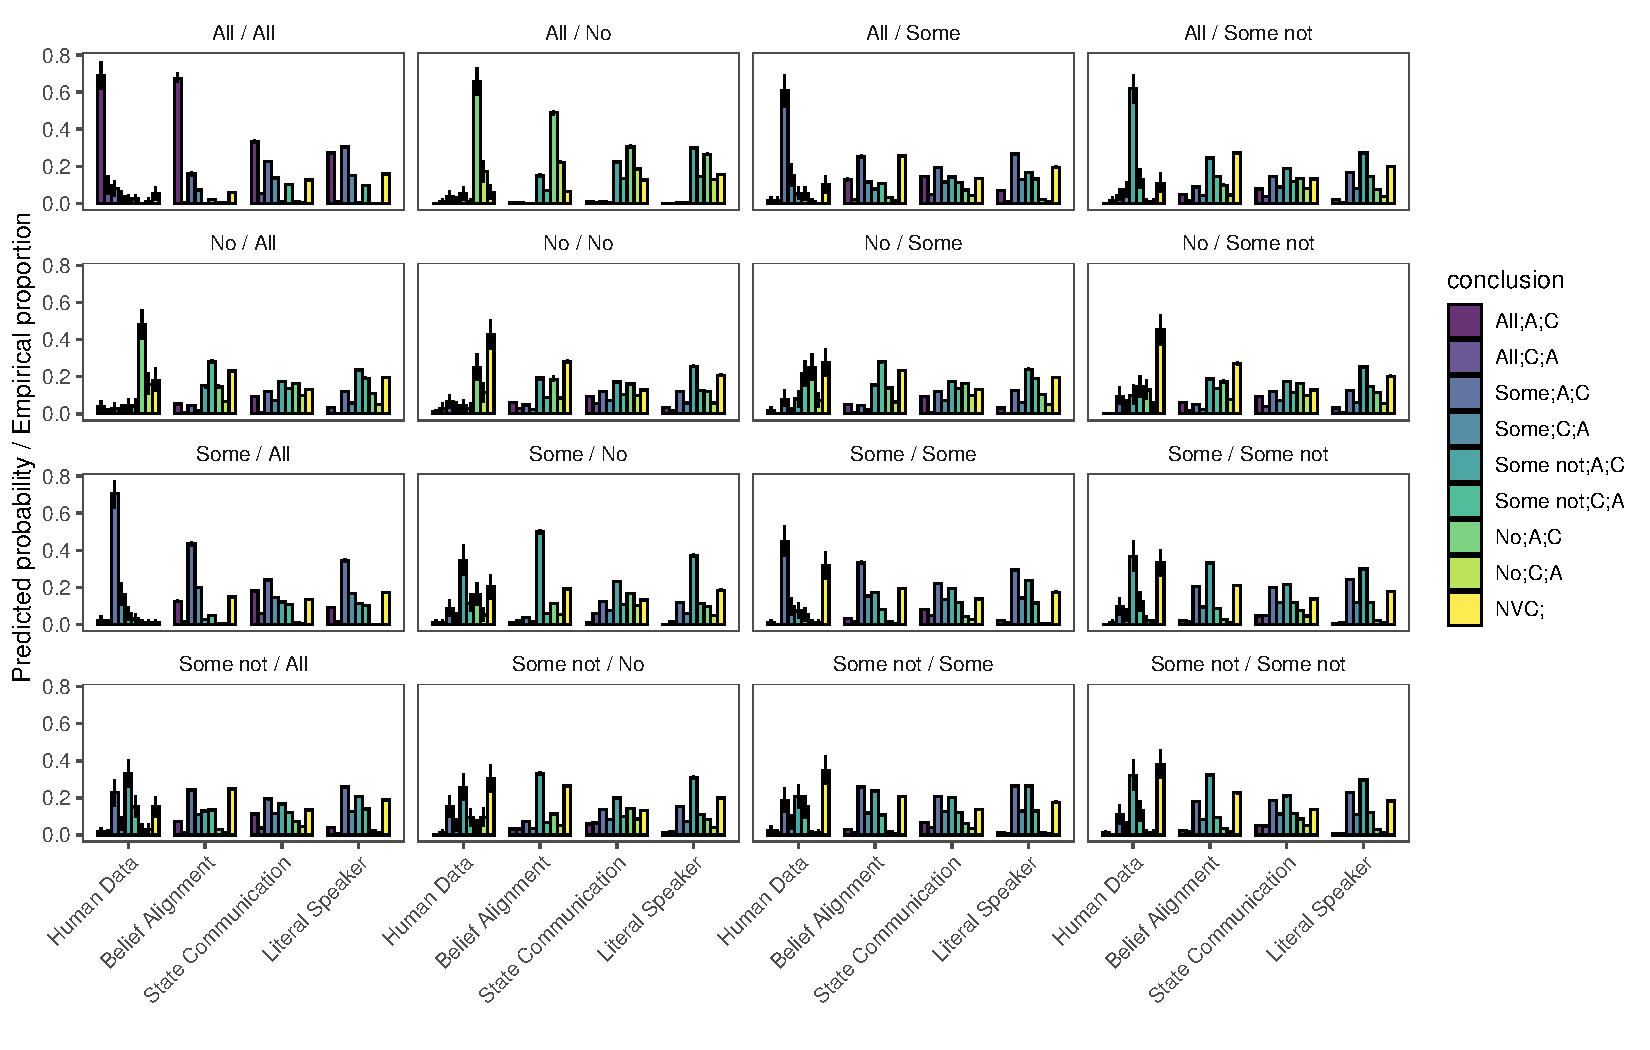
\includegraphics[width = \textwidth]{figs/bda_rsa_bars_0params.pdf}
\caption{Model predictions and behavioral results for the 9 possible conclusions to 16 syllogisms. Syllogisms are of the form: \emph{\_\_ As are Bs. \_\_ Bs are Cs.} Error bars denote bootstrapped 95\% confidence intervals for the human data and 95\% Bayesian credible intervals for the model predictions.}
\label{fig:bars}
\end{figure}





%\paragraph{Model comparison}
%
%   
%
%\paragraph{Posterior predictive checks}
%
%\paragraph{Posterior on parameters}


%\newcommand{\rlgetvalue}[4]{\csvreader[filter strcmp={\mykey}{#3},
%             late after line = {{,}\ }, late after last line = {{}}]
%            {\datafoldername/#1}{#2=\mykey,#4=\myvalue}{\myvalue}}
            
% Here is a number: 
% \rlgetvalue{rsa_model_params.csv}{model_param}{M00_LIT_LIT_noise}{MAP}


\subsection{Comparison to other theories}

%\ndg{awk:}We found the model that explained the human syllogistic reasoning data set the best was that which produced conclusions by aligning a listener's beliefs with those of a speaker (who had their beliefs updating from the literal meaning of the premises).
Our modeling approach is a Computational or Rational Level of analysis model \cite{marr1982vision, anderson1990adaptive} that seeks to describe the computations that underly human syllogistic reasoning without stipulating a precise implementation of such a reasoning process. 
Many other theories of syllogistic reasoning instead consider the process by which a human reasoner solves a syllogism.
The two most influential theories of human syllogistic reasoning are the Mental Models Theory \cite{johnsonlaird2006we, khemlani2013processes} and the Probability Heuristics Model \cite{Chater1999}, each of which share features with our logic, probability, and pragmatics approach. 


\begin{figure}[t]
\centering
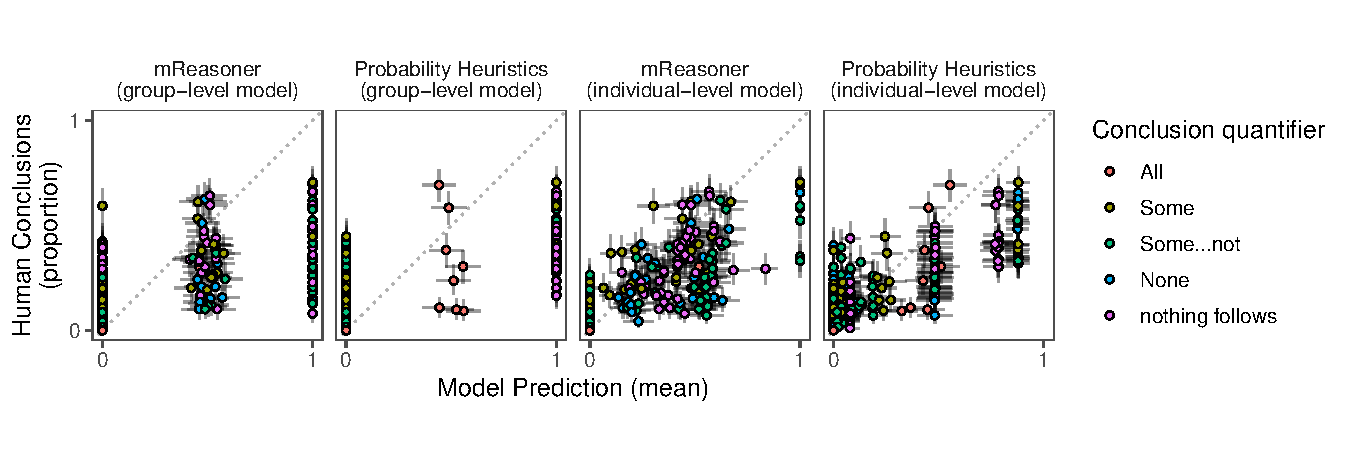
\includegraphics[width = \textwidth]{figs/alternative_model_scatters.pdf}
\caption{Performance of alternative theories. Each point represents an individual premise and conclusion pair. Group-level models use parameters that are fit to the group-level data. Individual-level models use parameters specific to individual participants. }
\label{fig:altModels}
\end{figure}

\subsubsection{Alternative models}

\paragraph{Mental Models}

The Mental Models Theory considers reasoning over a set of iconic models, in which individual entities are represented explicitly, not unlike our state space of Venn Diagrams. 
The reasoning process under this theory proceeds by first constructing a the mental model, proposing a conclusion that can be drawn from such a model, and then engaging in a search for counterexamples to that conclusion; if a counterexample is found, either the mental model is revised and the search for a conclusion continues or the reasoner concludes \emph{nothing follows}. 

Here we compare to a recent implementation of this theory \cite<the mReasoner model>{khemlani2013processes}, which is also probabilistic in nature (e.g., the model determines the number of objects to represent in the model by sampling  from a Poisson distribution). 
The model has four free parameters (canonically denoted $\lambda$, $\epsilon$, $\sigma$, and $\omega$): 
$\lambda$ determines the number of entities represented in the model, $\epsilon$ determines the kind of mental model constructed (either a canonical or non-canonical representation of the entities consistent with the syllogism; as described by \citeNP{bucciarelli1999strategies}), $\sigma$ denoted the probability of engaging in a search for counterexamples, and $\omega$ modulates the conclusion selection process that results when engaging in a search for counterexamples.  
%σ denotes the propensity of mReasoner to engage its search for counterexamples and ω specifies how to continue after a counterexample is found. With the proba- bility of ω, the conclusion quantifier is weakened and a new search for counterexamples starts.
\paragraph{Probability Heuristics} 

The Probability Heuristics model of \citeA{Chater1999} seeks to account for human syllogistic reasoning as a process of determining probabilistically valid (``p-valid'') conclusions, which can be approximated through a number of heuristics. 
Two heuristics generate candidate quantifiers for the conclusion, which use a notion of informativity for which \citeA{Chater1999} define a rank ordering: \emph{all} $>$ \emph{some} $>$ \emph{none} $>$ \emph{some...not}.  
The ``min-heuristic'' takes the quantifier of the least informative premise to be a potential conclusion quantifier and the ``p-entailment heuristic'' further allows for a quantifier that is entailed by the ``min-heuristic'' quantifier to also be a candidate quantifier for the conclusion (e.g., is \emph{all} is generated from the ``min-heuristic'', \emph{some} will be generated from the ``p-entailment heuristic''). 
A parameter (canonically referred to as $p_{ent}$) modulates which heuristic (min or p-entail) the reasoner uses to generate conclusions. 
A third heuristic (``attachment'') determines the ordering of the terms in the conclusion (A--C vs. C--A): this heuristic stipulates that the subject term of the conclusion should match the subject term of the least-informative premise, when allowable. 

Two more heuristics determine the confidence (or, probability) of each the candidate conclusions. 
Foremost, the ``max-heuristic'' stipulates the the probability of a candidate conclusion is proportional to the informativity of the most informative premise.
The ``O-heuristic'' additionally downweights conclusions that use the ``some...not'' quantifier.
In the implementation of this model that we use, these heuristics are parameterized by 4 parameters, which govern the confidence placed in conclusions of each of the four quantifiers (all, some, some...not, and none).

\subsubsection{Quantitative comparison}

To compare the quantitative accuracy of these alternatives theories to our own, we analyze the results of a recent study of these theories which focused on modeling the behavior of individual participants in the syllogistic reasoning task \cite{riesterer2020models}.
This study explored the predictive capabilities of the mReasoner and Probability Heuristics theories by treating the parameters of the models as individual-level parameters which could vary among participants (as well as the group-level version of the model, in which a single set of parameters governs the behavior of the population of participants).
The parameters of these models were fit to the same data set from \citeA{ragni2019does} that we modeled above with the Rational Speech Act models.\footnote{The predictions of these models were accessed via the companion repository to the paper: \url{https://github.com/nriesterer/cogsci-individualization}.}

Since \citeA{riesterer2020models} focus on predictive accuracy of the models for individual behavior, their implementation of the Probability Heuristics model treats the five model parameters as binary (0 or 1). This focus on predictive accuracy means that if a participant uses a heuristic $<50\%$ of the time, the best predictions that could be made would result by setting the corresponding parameter to 0. 
To examine the predictions of these theories in a manner more comparable to our analysis of the Rational Speech Act models, we treated the predictions of these alternative models for individual participants similar to how we treated the behavioral responses of individual participants. 
We constructed bootstrapped 95\% confidence intervals for the model predictions by resampling with replacement the predictions for each unique syllogism and conclusion. 



\begin{center}
\begin{table}[h]
\centering
\pgfplotstabletypeset[sci zerofill,
    col sep = comma,
    every head row/.style={before row = \toprule, after row = \midrule},
    every last row/.style={after row = \bottomrule},
    columns/model/.style={string type, column name={Model}, column type = l},
    columns/r/.style={string type, column name={$r$}, column type = l,  sci sep align, precision=2},
        columns/r2/.style={string type, column name={$r^2$}, column type = l,  sci sep align, precision=2},
   columns/mse/.style={fixed, column name={MSE}, column type = l, dec sep align, precision=3},	      
   columns/nParameters/.style={string type, column name={Parameters}, column type = l,  sci sep align, precision=3},
     ]{csv_to_tex/allModels_stats_0paramPriors.csv}\caption{Summary statistics for the RSA and alternative models. Alternative models were fitted to both group level data and individual level data. Individual-level variants use a new set of parameters for each individual participant in the data set ($n=139$).}\label{tab:altStats}
\end{table}
\end{center}

% The comparison of these model predictions to the behavioral data for each syllogsim and conclusion is shown in . 

The mReasoner and Probability Heuristics models with parameters fit globally to the whole data set (group-level models) perform quite poorly overall (Figure \ref{fig:altModels}). 
The models largely make categorical predictions (1s or 0s) whereas the aggregated human data is graded.
With parameters fit to individual participants and predictions aggregated, the mReasoner and Probability Heuristics models perform quite a bit better and comparable to our Rational Speech Act models in terms of their correlation and mean squared errors.
The individual-level parameterization of the models use a different set of parameters for each of the 139 participants in the task, however, yielding a total number of parameters that is 1-to-2 orders of magnitude larger than the the group-level versions of these models and our Rational Speech Act models (Figure \ref{fig:altModels}).\footnote{We discuss model complexity here in a coarse-grained manner. The PHM parameters in the \citeA{riesterer2020models} implementation are binary and thus do not add to model complexity in the same way as continuous parameters do. Still, we think that the approximate complexity of the models can be appreciated by their order-of-magnitude difference in the number of the parameters.}
These results suggest that these alternative theories encode process-level hypotheses that may be well-suited to model an individual participant's reasoning behavior, but are insufficient to adequately describe the computational problem that human reasoners are aiming to achieve. 

%The group-level version of the mReasoner model has 4 parameters and PHM has 5.
%Their corresponding individual-level models have 556 ($4\times 139$) and 695 ($5 \times 139$) parameters.
%Our Rational Speech Act models have approximately 10 parameters.





%For the : these models  and our Rational Speech Act models (~10 parameters).


%  as models of individual reasoners 

% \section{Experiments}

\section{General Discussion}

Reasoning with syllogisms sits at the intriguing intersection of language and logic. 
Syllogisms are a logical system, but they are expressed using natural language quantifiers and invite natural language inferences. 
We developed and tested a family of probabilistic models of syllogistic reasoning that incorporate a logical semantics with a generative model of situations and then formalize how considerations of pragmatic informativeness could affect the selection of conclusions.
We found that conclusions selected by participants were best explained by a model that chose its conclusion from a syllogism by reasoning about how well that conclusion would align a naive listener's beliefs with those of their own. 
We next discuss the modeling approach in more detail, including how it can be extended to account for other phenomena in syllogistic reasoning, as well as implications of our findings in the context of other work on pragmatic reasoning with syllogisms.

Our proposal is that human syllogistic reasoning is part logical, part probabilistic, and part pragmatic. Our theory is a rational model that articulates the functional problem human syllogistic reasoning is aiming to solve, which is at its core a problem of communication. Our work builds on the goal articulated by \citeA{Chater1999} of building a rational model of syllogistic reasoning, and we do so without positing any heuristic solutions to the inference problems. Our model is also deeply connected to the Mental Models approach \cite{johnson1975models, johnson2015logic} in that the states of affairs that our model reasons over are mental models of the world. 
One subtle difference is that a Mental Models theory would typically reason about tokens or instances of categories whereas our model reasons about types. 

%\mht{add connection to Oaksford \& Chater, mental models... tradition of probabilistic reasoning... }
We contrasted two mechanisms by which pragmatic considerations can enter into the production of conclusions: one based on informatively describing a particular state (or, Venn diagram) and one based on conveying the reasoner's entire belief distribution over states (i.e., their distribution over possible Venn diagrams). 
The results, both quantitatively and qualitatively, provide overwhelming evidence that it is the latter notion of belief alignment which most closely tracks human reasoning patterns. 
This formalization of pragmatic considerations differs sharply from previous perspectives on pragmatics in syllogistic reasoning.
Most notably, \citeA{Roberts2001} explored the predictions of an approach most similar to our State Communication model: how a reasoner would choose Gricean-enriched quantifiers (e.g., \emph{some} which implies not all $\neg \forall$) for each of the possible states (Venn diagrams) implied by the premises (which could have also been pragmatically enriched). 
Consistent with the observations of \citeA{Roberts2001}, such a State Communication model fails to provide any quantitative improvement across the data set, while our Belief Alignment does.
%and does not articulate a rational basis for producing the \emph{nothing follows} response.


% Analyzing the states (diagrams) in isolation has a number of flaws.
%First, \mht{insert qualitative phenomenon that emerges from belief alignment}.

%They looked at logic-based accounts in which the quantifiers \emph{some} and \emph{some...not} are interpreted in a Gricean fashion (e.g., \emph{some} pragmatically implies \emph{not all}, $\neg \forall$) and analyzed 

%Second, it %\mht{loop in Guerts natural logic?}


A major shortcoming of extant approaches to syllogistic reasoning is that they do not provide a clear and interpretable mechanism by the which the conclusion that \emph{nothing follows} can be rationally produced \cite{riesterer2020modeling}. 
%Our modeling approach to pragmatic speakers also provides a clear, interpretable mechanism by which the conclusion that \emph{nothing follows} option can be rationally produced, a shortcoming of extant approaches to syllogistic reasoning  
We formalized \emph{nothing follows} as a semantically vacuous statement which does nothing to update the listener's beliefs. 
This kind of utterance is, in the semantic sense, always true, and thus the Literal Speaker produces this utterance with constant probability.\footnote{Technically, the literal speaker produces this vacuous utterance with probability inversely proportional to the number of conclusions that are semantically compatible with the premises, which will vary based on the logical (in)validity of the syllogism.}
The Belief Alignment speaker, by contrast, selects utterances in order to convey their full beliefs about the state to the listener. 
When their beliefs are not substantially changed by hearing the premises (e.g., with certain logically invalid syllogisms), the speaker will have a positive incentive to say \emph{nothing follows} as that utterance would correspondingly not alter the listener's beliefs, leading to strong alignment between speaker and listener beliefs. 
To our knowledge, this formalization is the first substantive hypothesis about how the \emph{nothing follows} conclusion can be rationally produced in the syllogistic reasoning task.
%\mht{change last sentence:: This model serves as a substantial contribution to the syllogistic reasoning literature, as the formalization and treatment of the \emph{nothing follows} conclusion is something that has been missed from extant proposals \cite{riesterer2020modeling}}.

Our approach to syllogistic reasoning is at its core a Bayesian approach, where the premises of a syllogism update a reasoner's prior beliefs about the relationship between three properties. 
In our modeling, we did not assume anything substantive about these prior beliefs, except that they were constant across all syllogisms. %, and we used Bayesian data analysis to infer the prior beliefs used in the reasoner model, a kind of ``descriptive Bayesian'' approach \cite{tauber2017bayesian}.
Prior beliefs can, however, form the basis for formalizing hypotheses about how the content of the syllogism (i.e., the content of the particular terms: A, B, C) affects reasoning, a topic known that ``belief bias'' that has been of interest to psychologists for decades \cite{Oakhill1989, Oakhill1993, Cherubini1998}.
For example, \citeA{tessler2015understanding} found that some content effects in syllogistic reasoning could be captured by empirically measuring the relevant prior beliefs and using them in a model similar to that presented here.
Further work should look to these prior beliefs to formalize hypotheses about how world knowledge rationally affects reasoning, which could speak to outstanding debates about whether these effects should be considered a ``bias'' \cite<e.g.,>{Klauer2000, Garnham2005, Dube2011}. 

Our model uses the literal, natural language semantics of the premises of the syllogism to update the model's prior beliefs. 
It is straightforward to extend our approach to reasoning with other explicit quantifiers (e.g., \emph{most} and \emph{few}; see e.g., \citeNP{tessler2014some}, cf., \citeNP{geurts2003reasoning}).
Additionally, syllogisms that appear in natural discourse often make use of implicitly quantified, generic statements (e.g., \emph{Taxes on the wealthy will be modified}; see also \citeNP{khemlani2008syllogistic}); our approach could naturally be expanded to incorporate recent advances in the computational semantics of generics to account for syllogistic reasoning about generic premises \cite{tessler2019language}. 
Finally, this model could be used to consider the implications of pragmatic reasoning on the interpretation of the premises. 
Such a pragmatic interpretation model could be constructed as a standard Rational Speech Act pragmatic listener \cite{Frank2012a, goodman2016pragmatic, scontras2018probabilistic}; that is, treating the listener component of the model as a listener who reasons about why a speaker produced the premises that they did, where the speaker decides what utterance to produce in order to convey information about the state (or, belief distribution) to a naive literal listener.  %is the kind of pragmatic speaker we have considered in this paper, who 
Indeed, we have explored several versions of this kind of pragmatic model in the course of this project (described briefly in the Appendix) but found that no model extension we tried provided a substantially better quantitative fit to Ragni et al. (2019) data than the model that interprets the premises literally as we presented.\footnote{
Specifically, we formalized pragmatic listener models that interpret the premises from a rational speaker who wants to convey information about the full state as well as a speaker who wants to convey information about a number of different Questions Under Discussion \cite{Roberts2004QUD}, in which the speaker only cares about conveying information about the $A, C$ terms of the state; see also \citeNP{tessler2014some} for yet a different formulation of pragmatic interpretation of premises which achieves a comparable fit to that presented here.
}
We do not take this null result as evidence that pragmatics does not enter into the interpretation process of a syllogism.
We have only considered one particular experimental protocol and data set (from Ragni et al., 2019), where participants were presented with all 64 syllogisms, which potentially reveals the generative process of the syllogism (parametric recombination of quantifiers and term orders) and perhaps induces a more logical analysis of the syllogisms.
As well, the participants were from Western, educated, industrialized, rich, democratic societies, a feature not shared with most other human beings \cite{henrich2010most}. 
% \mht{confirm the participants of Ragni et al. were WEIRD?}.
Reasoning with syllogisms varies appreciably across individuals \cite{galotti1986individual, bacon2003individual} and substantially so in illiterate persons \cite{dias2005reasoning}.
In other contexts or populations, we may see that reasoning with syllogisms as a special case of reasoning about an argument or a riddle \cite<cf.>{luria1976cognitive, Ong1982}. 
Extending our modeling approach with a pragmatic interpretation component will be important for analyzing such behavior. 

% Aristotle invented syllogisms in order to tame -- to make more precise -- the human capacities for reasoning.
% Cognitive psychologists turned formalism back on itself and created a measuring stick by which to evaluate human reasoning. 

We articulate the verbal reasoning machinery that underlies the human capacity to reason with deductive arguments. 
This machinery is composed of three ingredients: logic, probability, and pragmatics. 
The combination of logic and probability enables us to reason about situations we have not experienced, but could encounter in the future.
The conclusions we draw are not just those that are plausible, however.
An agent needs to be posited at the other end of the line so that a conclusion makes sense; so that an argument may convince!

%\mht{need a final punch}
%\mht{this is approximately a copy-paste job from our cogsci syllogism paper}
%In our framework, a syllogism is seen as an argument given as a part of discourse between interlocutors. Indeed, this is how syllogisms were used in the time of Aristotle and in the long tradition of scholastic philosophers since. 
%The results of the pragmatic Bayesian reasoner models recast the ancient idea that human reasoning behavior is as much reason as it is human. 
%
%

%Our model is of a speaker who produces the conclusion to draw from the syllogism by reasoning about how a naive listener would interpret that conclusion, where the objective is to align the belief distribution of the listener to that of the speaker (formalized as a KL-divergence between distributions).


 


%Our approach to pragmatics differs from theirs in a number of important respects.
%Foremost, in our model, pragmatic enrichment of quantifier meanings is not an all-or-nothing phenomenon.
%Instead, the implications of pragmatics emerge probabilistically via Bayesian social reasoning, where a speaker reasons about how their words will affect the beliefs of a naive listener; these beliefs are probabilistic in nature, and the resulting pragmatic enrichment is a gradient phenomenon. 
%Second, we contrasted treatment of the pragmatic production of conclusions component of the model relies upon the idea that the reasoner is trying to select the conclusion that best conveys her belief distribution about the answer to the QUD (i.e., the AC part of the Venn diagram); in doing so, the reasoner is able to rationally produce \emph{nothing follows} in situations where her belief distribution is not substantially different than her prior beliefs about the QUD. 
%
%
%This probabilistic treatment of pragmatic reasoning has two effects: (i) \emph{some} does not necessarily imply $\neg \forall$ and (ii) the interpretations of \emph{some A are B} and \emph{some A are not B} are not equivalent (contra the treatment in \citeNP{Roberts2001}).
%
%
%Second, we introduce the idea that the syllogistic reasoning task presents a particular Question Under Discussion (QUD) which can alter the pragmatic enrichments that alter the literal meaning of the premises in a syllogism; in particular, the syllogism introduces the \textsc{AC} QUD (``what is the relation between A and C?'' ), which invites the listener to weight the evidence for a particular conclusion from the current syllogism in the space of possible syllogisms. 



\newpage

\bibliographystyle{apacite}
\bibliography{syllogism}

\newpage 

\appendix

\section{Appendix: Pragmatic interpretation of premises}

%\subsubsection{}

Understanding language often involves reasoning not only about the literal meaning of what was said but about why an interlocutor (the speaker) would bother to say what they said, which can lead to enriched interpretations beyond the literal meanings. 
We can formalize this reasoning through a series of Bayesian models that recursively reason about one another, as developed in the Rational Speech Act (RSA) framework \cite{Frank2012a, goodman2016pragmatic, scontras2018probabilistic}.
Concretely, we can describe a pragmatic listener $L_1$ who reasons about a speaker $S_1$ who produces utterances in order to convey information to the literal listener (Equation \ref{eq:L0premises}):

\begin{align}
L_1(s \mid u_1,  u_2)& \propto  P(s)\cdot S_1(u_1, u_2 \mid s)  \label{eq:L1} \\ 
S_1(u_1, u_2 \mid s) &\propto  \exp [ \alpha_1 \cdot \ln L_0(s \mid u_1,  u_2)]  \label{eq:S1}
\end{align}

The definition of the pragmatic listener (Equation \ref{eq:L1}) mirrors that of the literal listener (Equation \ref{eq:L0}) except in that the likelihood is defined as the probability that a speaker $S_1$ would produce utterances (premises) $u_1$ and $u_2$ given a state $s$.
Following standard practice in RSA modeling, the speaker is a soft-max rational agent (with degree of rationality $\alpha_1$) who produces utterances in order to convey information about the state $s$ to the literal listener (formalized by the negative surprisal of state given the utterances: $\ln L_0(s \mid u_1,  u_2)$).

\paragraph{Alternative utterances}
The proportionality in Equation \ref{eq:S1} implies a normalization over a set of alternative utterances (i.e., the set of sentences that the speaker could have produced); in our case, the set of alternative utterances amounts to a set of alternative syllogistic premises that a speaker could have produced. 
There are at least three sets of alternative premises that are \emph{a priori} plausible and we tested models using each of: (1) alternative premises that have the same ordering of terms (i.e., syllogisms of the same form, or ``figure''), but whose quantified relation between the terms could be different (e.g., if the speaker says \emph{All As are Bs / All Bs are Cs}, the alternative set is the set of syllogisms of the form \emph{Q As are Bs} / \emph{Q Bs are Cs} where $Q \in \{all, some, \emph{not all}, none\}$); (2) alternative premises that differ either in the quantified relation between terms or the ordering of the terms, but not both (i.e., utterances with an edit-distance of 1); (3) the maximal set of alternative premises in which the quantifier and the ordering of terms could be different.

\paragraph{Question Under Discussion (QUD)}
When deciding what to say, speakers may choose their utterances to convey information about a particular topic of relevance and listeners may assume that speakers had a particular topic of relevance in mind when interpreting the utterances heard. 
We formalize this topic as a Question Under Discussion (or, QUD), which acts as a function that projects the state space onto a lower-dimensional representation of the state space \cite{Roberts2004QUD, kao2014nonliteral}.
Though QUDs may not be the explicit question asked of a person \cite<e.g.,>{}, in the context of a syllogistic reasoning problem, the most natural QUD is the explicit question asked of participants: What relationship between As and Cs follows from the premises? \cite{tessler2014some}
In particular, we considered the QUD when interpreting the premises of a syllogism (\emph{As are Bs}, \emph{Bs are Cs}) to be about the A--C relationship. 
In our model, this QUD function acts by transforming a three circle Venn diagram (A, B, C) into a two circle diagram (A, C): $Q(\{A,B,C\}) = \{A,C\}$.
%Example results of this transformation can be seen in Figure \ref{fig:lit_state_qud}(ii). 


The pragmatic listener who interprets the premises relative to this QUD is given by a set of equations:

\begin{align}
L_1(s \mid u_1,  u_2, Q)& \propto  P(s)\cdot S_1(u_1, u_2 \mid s, Q)  \label{eq:L1q} \\ 
S_1(u_1, u_2 \mid s, Q) &\propto  \exp [ \alpha_1 \cdot \ln L_0(Q(s) \mid u_1,  u_2, Q)]  \label{eq:S1q} \\
L_0(Q(s) \mid u_1,  u_2) & = \sum_{s' \in \mathcal{S}}  \delta_{Q(s)=Q(s')} \cdot L_0(s'\mid u_1,  u_2) \label{eq:L0q}
\end{align} 
%\mht{is this the best way to write out the QUD model?}



\end{document}
